% !Mode:: "TeX:UTF-8"
%!TEX program  = xelatex

\documentclass[bwprint]{gmcmthesis}

\usepackage{graphicx}
\usepackage{tabularx}
\usepackage{caption}
\usepackage{float}
\usepackage{setspace}


\usepackage[framemethod=TikZ]{mdframed}
\title{出血性脑卒中预后预测:集成静态模型和时序模型}
\baominghao{} %参赛队号
\schoolname{}%学校名称
\membera{} %队员A
\memberb{} %队员B
\memberc{} %队员C
\begin{document}

 %生成标题
 \maketitle

 %填写摘要
\begin{abstract}

出血性脑卒中是最严重且最难治疗的疾病之一,但受限于医疗手段的不足、检查会导致损伤的问题以及相关研究尚不成熟,治疗和诊断非常困难。本文使用出血性脑卒中患者的静态数据和时序数据,尝试通过投票拟合机、传统机器学习、深度学习、群智能算法、集成学习,进行临床智能诊疗建模。

针对问题1:a)本文提出投票拟合机选取最优的拟合曲线模型,为每个患者的血肿数据筛选出残差最低的模型,通过牛顿下山法获取48小时内血肿扩张事件发生的时间点,记录血肿扩张发生的标签和时间;b)本文通过比较逻辑回归(LR)、随机森林(RF)、XGBoost(XGB)、LightGBM(LGBM)、支持向量机(SVC)、多层感知器(MLP)这些模型,使用合成少数类过采样技术(SMOTE)处理后的数据进行训练和比较,选择F1得分最高的MLP模型,通过网格搜索和k折交叉验证最优化超参数后,进行血肿扩张发生概率的预测。

针对问题2:a)本文通过观察数据分布,选择使用高斯函数拟合出一条全体患者水肿体积随时间进展曲线,计算同真实值的残差;b)本文通过比较K-Means(K 均值聚类)、Hierarchical Clustering(层次聚类)、Birch(平衡迭代规约和聚)、Spectral Clustering(谱聚类)这些模型,使用网格搜索和K折交叉验证最优化超参数后进行训练和比较,选择Silhouette coefficient(Silhouette 系数)最大的K均值聚类进行5个聚类中心的分组,每组通过投票拟合机选择最优的拟合曲线进行拟合,计算与真实值的残差;c)本文使用多元广义线性模型(GLM),将治疗方法分为单一治疗方法和组合治疗方法两类,分别对标准化后的水肿体积特征数据进行分析;d)本文使用两类治疗方法分别对血肿趋势和水肿趋势进行单因素方差分析,对血肿趋势和水肿趋势使用投票拟合机选取残差最小的函数模型进行曲线拟合。 

针对问题3:a)本文基于SMOTE采样后的数据,使用反向传播神经网络模型(BP神经网络模型)训练,通过蚁群算法优化(ACO)模型的超参数,对患者的mRS进行预测;b)本文基于SMOTE采样后的数据,将具有时间属性的数据与不具时间属性的数据分组,具有时序属性的数据导入模糊时间间隔的长短期记忆网络模型(LSTM)中,将不具有时序属性的数据导入BP神经网络模型中
同时使用ACO优化上述两个模型,最后使用投票模型将两个模型融合为预测模型,对患者的mRS进行预测;c)本文基于SMOTE采样后的数据,将变量分为有序变量与无序变量,借助Shapiro-Wilk 分布检验,Kruskal-Wallis H 检验, Kolmogorov-Smirnov
分布检验,分析变量与90天mRS的相关性。 

\keywords{投票拟合机\quad  传统机器学习\quad   深度学习\quad  群智能算法\quad  集成学习\quad}
\end{abstract}

\pagestyle{plain}

%目录 不推荐加
%\tableofcontents

\section{绪论}

\subsection{引言}

脑出血是卒中中最严重且最难治疗的类型之一。每年全球有近2000万例新发卒中病例,其中大约有20\%属于脑出血类型。具体而言,在所有脑卒中中,出血性脑卒中的发病率为10-15\%。然而,即便存在如此庞大的患者群体,出血性脑卒中目前也缺乏有效和多样化的治疗方法,而且患者在急性期内的病死率高达45-50\%。这给社会和患者家庭带来沉重的健康和经济负\cite{cordonnier2018intracerebral}。

\begin{figure}[!h]
\centering
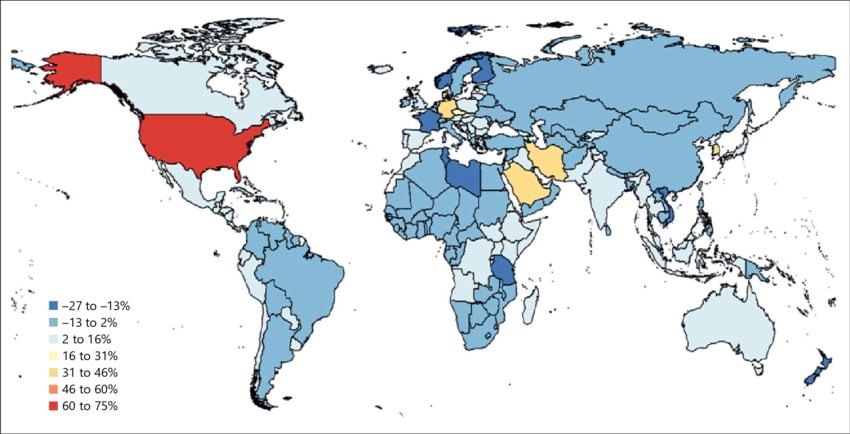
\includegraphics[width=.7\textwidth]{fig_me/问题背景.png}
\caption{1990年至2013年间,因出血性脑卒中引起的年龄标化患病率的百分比变化\cite{feigin2015atlas}}
\end{figure}

值得高兴的是,医学影像技术的进步为监测出血性脑卒中后脑组织的变化提供了强大工具。同时,人工智能技术在急性脑卒中影像等医疗领域的应用迅速增长,并在提高急性脑卒中患者治疗效果方面发挥着关键作用。早期识别急性脑卒中对于迅速采取干预以降低患者病情恶化和死亡率至关重要。人工智能可以在脑卒中治疗的各个方面提供帮助,包括梗死或出血检测、分割、分类、大血管阻塞检测、Alberta中风早期CT评分,以及预测。特别是新兴的卷积神经网络等人工智能技术显示出在这些基于影像的任务中高效准确的潜力\cite{soun2021artificial}。

在实际的应用中,可以结合影像数据、患者信息、治疗数据等构建智能诊疗模型,利用机器学习技术,甄别出导致出血性脑卒中预后不良的危险因素,实现个性化疗效评估和预后预测。血肿扩张是预后不良的重要危险因素之一,在出血发生后的短时间内,血肿范围扩大甚至可以危及患者的生命。因此,预测出血性脑卒中患者血肿扩张风险对于改善患者预后具有重要意义。此外,血肿周围的水肿是脑出血后继发性损伤的标志之一,是出血性脑卒中的另一个重要关键事件。因而研究血肿周围水肿发生及演进规律对于改善患者预后具有具有关键价值\cite{wagner2004hematoma,zheng2016mechanism}。

\subsection{问题的提出}
本文围绕出血性脑卒中预后,明确导致预后不良的危险因素,依次提出如下问题:

\subsubsection{问题一:血肿扩张风险相关因素探索}

对出血性脑卒中患者的血肿扩张风险精确预测,不仅能能够保障患者的生存质量,还能为后续的预后预测提供信息参考。

\subsubsection{问题二:血肿周围水肿的发生及进展探索}

进一步探索治疗干预和水肿进展的关联关系,可作为后续预后预测的信息指引。

\subsubsection{问题三:出血性脑卒中患者预后预测}

基于已知信息,准确预测预后,对于实现个性化疗效评估和改善预后具有重大意义。

\section{模型假设}
\begin{itemize}
\item 假设所有患者的影像数据是真实无误的;
\item 假设医院统计患者的治疗数据不存在笔误;
\item 假设原始数据已进行过初步的数据预处理,没有异常样本。
\end{itemize}

\section{问题分析}
\subsection{血肿扩张风险相关因素探索}

21世纪以来,尽管科技迅猛发展,世界医疗水平依旧难以满足社会需求。在社会节奏不断加快、环境日益恶化的情况下,人们生活压力与日俱增,很多人生活规律紊乱,脑卒中患者日益增多。在出血性脑卒中诊断过程中,有一个几个重要的指标是血肿是否发生扩散,何时发生扩散,而困扰脑卒中诊断的一个方面是相关医疗手段少、专业医生缺乏;第二个方面是诸多检查对患者身体造成一定的损伤,无法在较少时间间隔内对同一个人采样,总采样次数也较少;第三个方面则是相关研究尚未成熟,在众多的医疗检查数据中,混杂着很多因素对于分析血肿是否发生扩散、多大概率发生扩张、何时扩张这个问题造成干扰。为此,本文将该问题分为以下两点,并在所提供的数据集上进行了分析。

a)通过分析课题所给患者的血肿相关影像数据,分析出前100例患者是否在发病后48小时之内发生血肿扩张,并判断发生血肿扩张的患者的血肿扩张时间。

b)分析患者个人史,疾病史,发病相关指标,首次影像检查结果等变量,探讨患者发生血肿扩张的概率,并建立一个由上述变量到发生血肿扩张概率的模型,计算并记录前100例患者的血肿扩张发生概率。

\subsection{血肿周围水肿的发生及进展探索}

在人体组织特性下,发生血肿往往伴随着水肿的发生,而水肿的发生容易造成突发性颅压增大,是继发性损伤最关键的因素,同时水肿又反过来影响血肿的发展,也影响治疗方法的制定,所以,准确的分析血肿周围水肿的发生及进展是一个重要的课题,血肿周围水肿是继发性损伤的潜在替代标志物,可能导致血肿治疗的预后不良。为此,本文将该问题分为以下四点,并在所提供的数据集上进行了分析。

a)通过分析课题所给患者的水肿相关影像数据,建立回归模型,构建一条全体患者水肿体积随时间进展曲线,并计算前100例患者真实值和所拟合曲线之间存在的残差。

b)由于小样本人群存在较强的个体差异,在上一点中分析的结果会极差,因此,需要探索患者水肿体积随时间进展模式的个体差异,将人群分为3-5个亚组,并构建不同人群的水肿体积随时间进展曲线,并计算前100例患者真实值和所拟合曲线之间存在的残差。

c)为了探索发生血肿周围水肿时恰当的治疗方法,需要从已有的治疗方法及对应患者的水肿体积进展模式数据中,探索不同治疗方法对水肿进展模式的影响,以完善医疗手段。

d)在上一点的基础上,需要探索血肿体积、水肿体积及治疗方法三者之间的关系,以指导治疗方法的制定。

\subsection{出血性脑卒中患者预后预测}

出血性脑卒中是一种严重的疾病,对患者的健康和生活质量有着重要影响。预测出血性脑卒中患者的预后可以帮助医生和患者制定合适的治疗方法、提供个体化的护理以及做出未来的决策。预测出血性脑卒中患者的预后可以帮助医生选择合适的治疗策略。例如,对于预后较好的患者可能会采取更积极的治疗方法;而对于预后较差的患者可能会采取保守治疗措施。此外,预测出血性脑卒中患者的预后可以指导康复规划。通过了解患者的预后情况,医生和康复团队可以制定个体化的康复计划,以帮助患者尽快恢复功能,提高生活质量。同时,预测出血性脑卒中患者的预后可以指导康复规划。通过了解患者的预后情况,医生和康复团队可以制定个体化的康复计划,包括物理治疗、语言治疗和认知康复等,以帮助患者尽快恢复功能,提高生活质量。为此,本文将该问题分为以下三点,并在所提供的数据集上进行了分析。

a)分析前100例患者的个人史、疾病史、发病相关指标以及首次影像结果与患者“90天mRS”指标的相关性,并构建预测模型,预测所有患者90天mRS评分。

b)分析前100例患者所有已知临床、治疗以及所有影像结果与患者“90天mRS”指标的相关性,并构建预测模型,预测含随访影像检查的患者90天mRS评分。

c)分析出血性脑卒中患者的预后“90天mRS”和个人史、疾病史、治疗方法及影像特征(包括血肿/水肿体积、血肿/水肿位置、信号强度特征、形状特征)等关联关系,为临床相关决策提出建议。


\section{血肿扩张风险相关因素探索模型的建立与求解}
\subsection{模型1a的建立与求解}
\subsubsection{相关模型}
\textbf{线性回归}是一种简单的回归方法,用于建立连续因变量和一个或多个自变量之间的线性关系。其公式为:

\begin{equation}
y = \alpha_0 + \alpha_1 x_1 + \alpha_2x_2 + \dots + \alpha_nx_n\
\end{equation}

\noindent 其中,$y$是因变量,$x_1, x_2, \dots, x_n $是自变量,$\alpha_0, \alpha_1, \alpha_2, \dots, \alpha_n$ 是回归系数。

\textbf{二次函数回归}是一种建立因变量和自变量之间二次关系的回归方法。其公式为:

\begin{equation}
y = \alpha_0 + \alpha_1x + \alpha_2x^2
\end{equation}

\noindent 其中,$y$ 是因变量,$x$ 是自变量,$\alpha_0, \alpha_1, \alpha_2$是回归系数。

\textbf{三次函数回归}是一种建立因变量和自变量之间三次关系的回归方法。其公式为:

\begin{equation}y = \alpha_0 + \alpha_1x + \alpha_2x^2+\alpha_3x^3\end{equation}

\noindent 其中,$y$ 是因变量,$x$ 是自变量,$\alpha_0, \alpha_1, \alpha_2,\alpha_3$ 是回归系数。

\textbf{指数函数回归}是一种建立因变量和自变量之间指数关系的回归方法。其公式为:

\begin{equation}y=\alpha_0+\alpha_1e^{x/\alpha_2}\end{equation}

\noindent 其中,$y$ 是因变量,$x$ 是自变量,$\alpha_0, \alpha_1,\alpha_2$ 是回归系数,$e$ 是自然对数的底。

\textbf{对数函数回归}是一种建立因变量和自变量之间对数关系的回归方法。其公式为:

\begin{equation}y=\alpha_0+\alpha_1\ln{x}\end{equation}

\noindent 其中,$y$ 是因变量,$x$ 是自变量,$\alpha0, \alpha1$ 是回归系数,$\ln$ 表示自然对数。

\textbf{三角函数回归}是一种建立因变量和自变量之间三角函数关系的回归方法,常见的有正弦函数和余弦函数。以正弦函数为例,其公式为:

\begin{equation}y=\alpha_0+\alpha_1\sin{x}+\alpha_2\cos{x}\end{equation}

\noindent 其中,$y$ 是因变量,$x$ 是自变量,$\alpha_0, \alpha_1,\alpha_2$ 是回归系数。

\textbf{牛顿下山法}(Newton's Method with Line Search)\cite{kov2018NumericalLA} 是一种常用的非线性优化方法,通过二次逼近来求解无约束非线性问题。其主要思想是在当前点处,构造一个二次函数模型,然后求出这个二次函数的最小值点作为下一个迭代点,如此不断迭代直到满足收敛条件。

下面是牛顿下山法的数学公式:

设 $f(x)$ 是需要求最小值的目标函数,$x_k$ 是第 $k$次迭代的点,则牛顿下山法的迭代公式为:

\begin{equation}
x_{k+1} = x_k + \alpha_k p_k
\end{equation}

\noindent 其中,$\alpha_k$ 是步长,$p_k$ 是下降方向(Descent Direction)。

对于下降方向 $p_k$ 的选择,牛顿下山法采用了牛顿方向(Newton Direction),具体而言,就是找到当前点处的海森矩阵(Hessian Matrix)$H_k$,然后以负梯度为右端向量,利用海森矩阵求解一个线性方程组,得到下降方向 $p_k$,即:

\begin{equation}
H_k p_k = -\nabla f(x_k)
\end{equation}

步长 $\alpha_k$ 的选择通常采用线性搜索或非线性搜索。在线性搜索中,$\alpha_k$ 可以通过一维搜索确定一个满足一定准则(如Armijo条件)的最优步长;在非线性搜索中,$\alpha_k$ 可以通过求解一个子问题来确定。
\subsubsection{模型建立}\label{6种回归的章节}
由于小样本人群中个体差异极大,本文对前100例患者的血肿体积-时间序列数据分别做函数拟合,由于每个患者的数据分布不同,本文设计了一种集成了上一节中提到的6种回归模型的投票拟合机,即针对每名患者的血肿体积-时间序列数据分别做6种拟合算法,然后通过投票机制,将得分最高的一种拟合算法作为该名患者的血肿体积发展曲线,该投票拟合机的物理结构如图~\ref{投票拟合机的物理结构}所示。

\begin{figure}[!h]
\centering
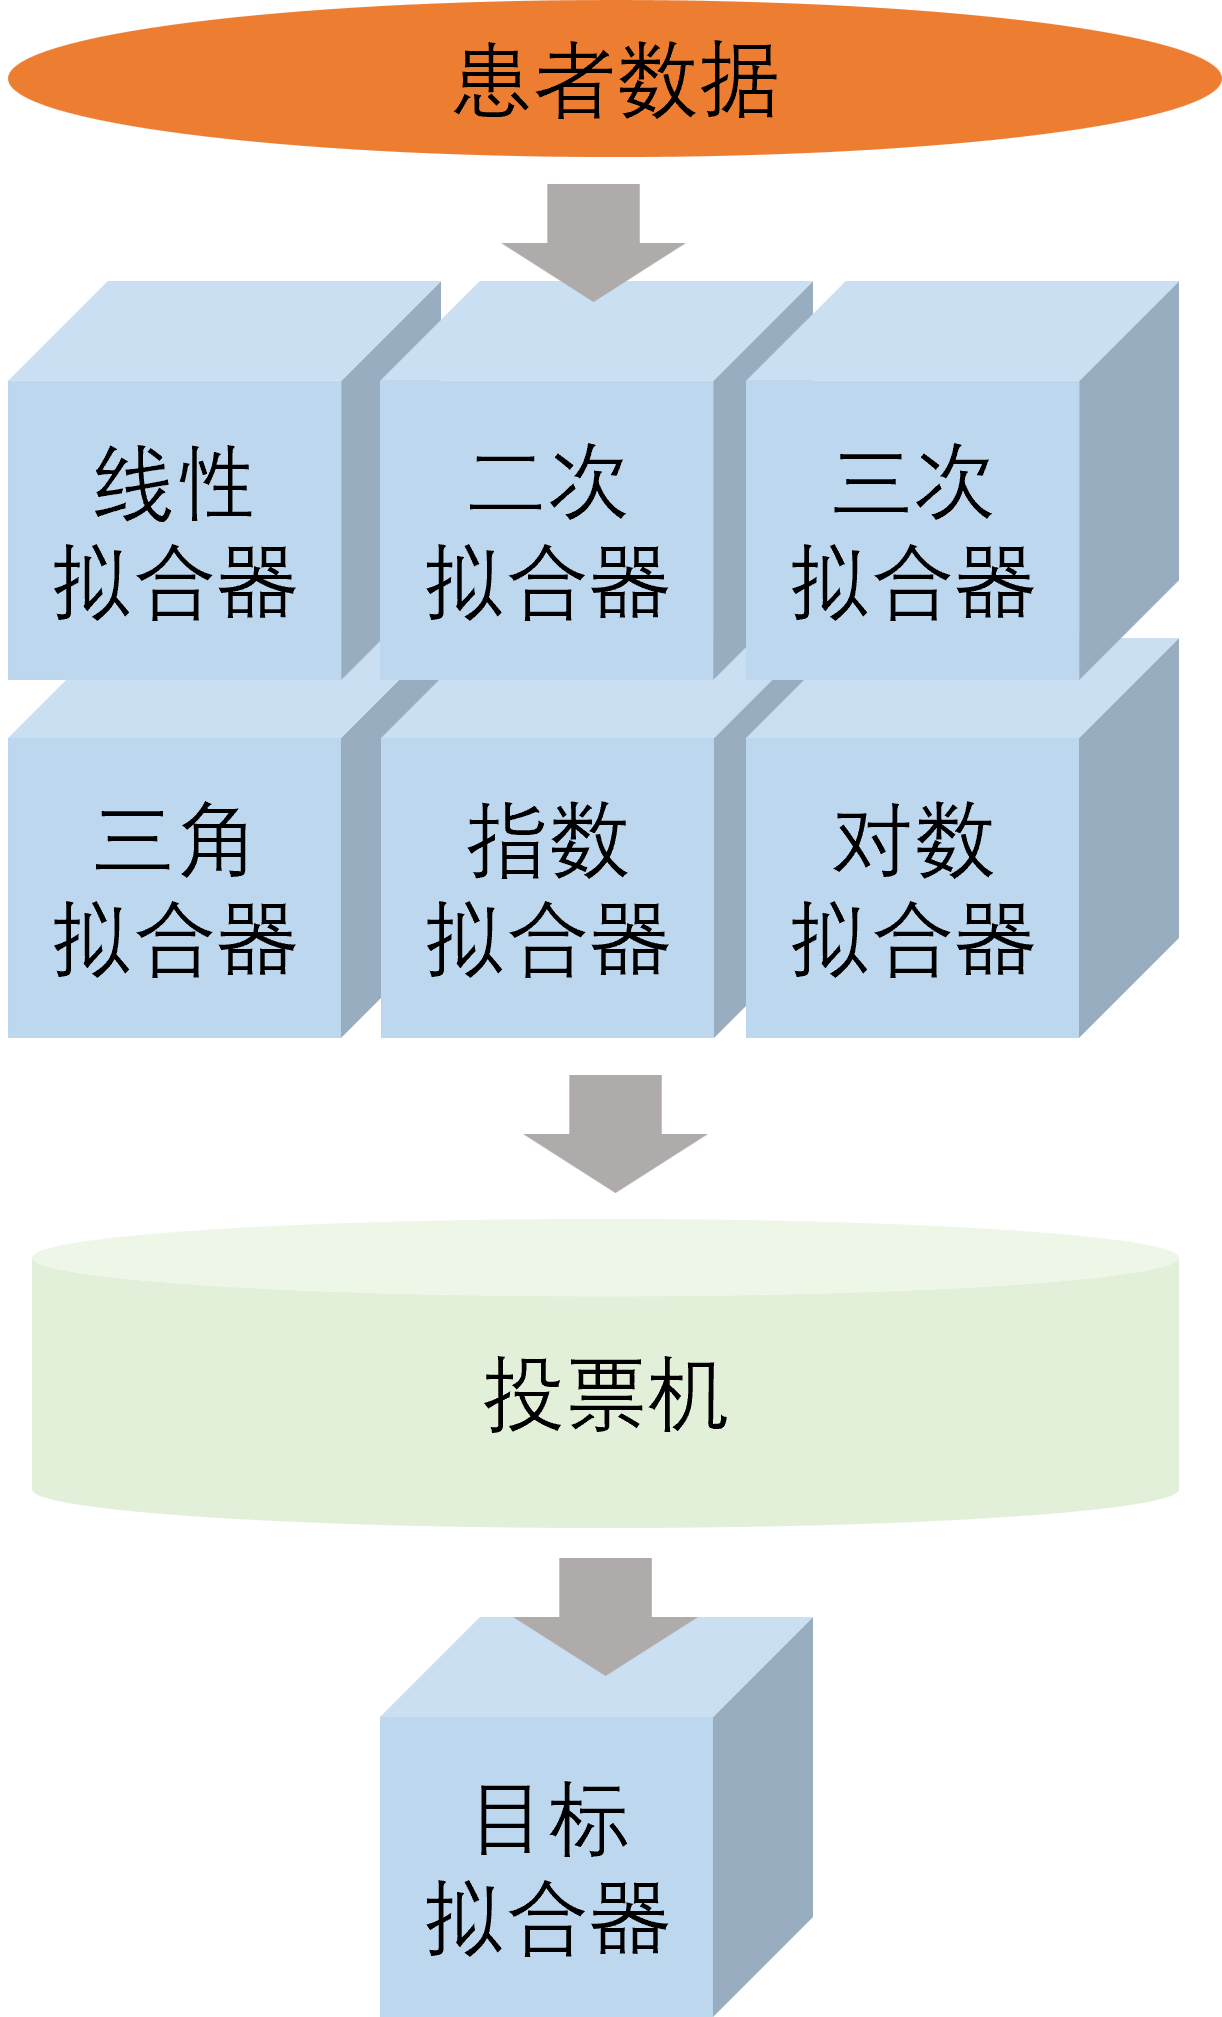
\includegraphics[width=0.3\textwidth]{fig_me/1a概念图.png}
\caption{投票拟合机的物理结构}
\label{投票拟合机的物理结构}
\end{figure}

在投票机内,本文设置了一个轮盘,初始化分数$R^2$为0,接下来,每转到一个拟合器,通过一下公式计算其得分$R^2$:
\begin{equation}
SST=\sum\limits_{i=1}^{n}(y_i-\overline{y})^2
\end{equation}

\begin{equation}
SSR=\sum\limits_{i=1}^{n}(\hat{y_i}-\overline{y})^2
\end{equation}

\begin{equation}
SSE=\sum\limits_{i=1}^{n}(y_i-\hat{y})^2
\end{equation}

\begin{equation}
R^2=\frac{SSR}{SST}=1-\frac{SSE}{SST}
\end{equation}

紧接着判断该轮得分$R^2$是否大于上一次转到的拟合器的得分$R^2$,若是,则替换目标拟合器,并继续转动,若否,则直接进行转动而不进行替换。

以此类推直到转盘在某一轮转动中转动了一圈并在该轮中没有更新目标拟合器,此时将该拟合器输出。

在确定拟合器后,使用该拟合器拟合出的曲线,根据牛顿下山法,求解下列两个函数:

\begin{equation}
Z_i(t)=HM\_v_{it}-HM\_v_{i0}-6,\, 0<i<=48
\end{equation}
\begin{equation}
Z'_i(t)=HM\_v_{it}-1.33HM\_v_{i0},\, 0<i<=48
\end{equation}

\noindent 其中,$i$表示第i位患者,$t$表示距离改该名患者发病时间的第$t$时刻,单位为小时,$HM\_v_{it}$表示第$i$名患者第$t$时刻的血肿体积大小,单位为毫升,$HM\_v_{i0}$表示第$i$名患者首次检查的血肿体积大小,根据题设,后续血肿体积比首次检查大了6ml或者大了33\%则判断为血肿扩张。

若上述求零点有解时,表示该名患者在48小时内发生血肿扩张,记录求解得到的时间;反之则无。


\subsubsection{模型求解}
本节根据问题要求,使用联表功能筛选出前100例患者的所有影像检查结果的HM\_volume列,即血肿体积,以及每个检查的具体时间,紧接着使用图~\ref{投票拟合机的物理结构}所示投票机,进行函数拟合,拟合机输出选择过程得分$R^2$参数如表~\ref{过程得分$R^2$}所示。

\begin{table}[!ht]
    \centering
    \caption{投票过程得分$R^2$(仅展示部分数据)}
    \label{过程得分$R^2$}
    \begin{tabular}{ccccccc}
    \hline
        ID & 线性回归 & 二次回归 & 三次回归 & 三角回归 & 指数回归 & 对数回归 \\ \hline
        sub001 & 0.8671 & 0.9779 & 0.9787 & 0.8486 & 0.867 & 0.455 \\ 
        sub002 & 0.8915 & 0.9861 & 0.9946 & 0.6013 & 0.9807 & 0.7795 \\ 
        sub003 & 0.3029 & 1 & 1 & 1 & 0 & 0.6544 \\ 
        sub004 & 0.8343 & 0.9989 & 1 & 0.4942 & 0.9928 & 0.8617 \\ 
        sub005 & 0.5461 & 1 & 1 & 1 & 0 & 0.8702 \\ 
        sub006 & 0.9266 & 0.9889 & 0.9943 & 0.7807 & 0 & 0.9817 \\ 
        sub007 & 0.8868 & 0.8876 & 0.9832 & 0.8427 & 0.8874 & 0.7195 \\ 
        sub008 & 0.0303 & 0.7839 & 1 & 0.9762 & 0.5508 & 0.2793 \\ 
        sub009 & 0.7057 & 1 & 1 & 1 & 0.9726 & 0.9308 \\ 
        sub010 & 0.5854 & 0.8489 & 1 & 0.5511 & 0.9744 & 0.9638 \\ \hline
    \end{tabular}
    
\end{table}

根据得分结果绘制前100名患者的回归曲线如图~\ref{函数拟合结果示意图}所示。
\begin{figure}[!h]
\centering
\includegraphics[width=1\textwidth]{fig_me/q11_20sub.png}
\caption{函数拟合结果示意图(仅展示部分数据)}
\label{函数拟合结果示意图}
\end{figure}

根据牛顿下山法求得结果如表~\ref{是否扩张及扩张时间}所示。
\begin{table}[!ht]
    \centering
    \caption{是否扩张及扩张时间(仅展示部分数据)}
    \begin{tabular}{ccc}
    \hline
        ID & 是否扩张(1是,0否) & 扩张时间(单位:小时) \\ \hline
        sub001 & 0 & ~ \\ 
        sub002 & 0 & ~ \\ 
        sub003 & 1 & 4.1497 \\ 
        sub004 & 0 & ~ \\ 
        sub005 & 1 & 15.3287 \\ 
        sub006 & 0 & ~ \\ 
        sub007 & 0 & ~ \\ 
        sub008 & 1 & 10.4402 \\ 
        sub009 & 1 & 13.0958 \\ 
        sub010 & 0 \\ \hline
    \end{tabular}
    \label{是否扩张及扩张时间}
\end{table}

\subsection{模型1b的建立与求解}
\subsubsection{相关模型}

\textbf{逻辑回归(LR)}\cite{Christodoulou2019ASR}是一种经典的线性模型,主要用于二分类问题。通过学习特征的权重参数,LR能够对输入特征进行线性组合,然后利用逻辑函数进行概率估计。由于模型本身的简洁性和高计算效率,使其成为进行早期数据探索的理想选择之一。

\textbf{随机森林(RF)}\cite{Keith2020RandomF}是一种集成学习模型,其性能提升来自多个决策树的投票结果。RF能够自动评估特征的重要性,具有出色的鲁棒性,特别适用于高维数据集,并在具有大量特征的数据分类问题中表现出色。

\textbf{XGBoost(XGB)}\cite{Ogunleye2020XGBoostMF}是一种梯度提升树模型,通过反复迭代地训练决策树以最小化损失函数。XGB在处理大规模数据集和高维特征空间时表现出色,其特点包括高效性和卓越的预测性能。

\textbf{LightGBM(LGBM)}\cite{Ke2017LightGBMAH}基于梯度提升框架,采用基于直方图的学习策略。它具有出色的速度和扩展性,特别适用于处理大规模数据集和高维特征的挑战。

\textbf{支持向量机(SVC)}\cite{Cervantes2020ACS}是一种监督学习模型,通过找到最优超平面将不同类别的数据点分隔开,并在最大化间隔的同时提高模型的泛化性能。SVC在处理大规模数据集时表现卓越。

\textbf{多层感知器(MLP)}\cite{yun2019radiomic,ma2019mri}是深度学习领域的经典神经网络模型,由多个神经元层组成。它具有学习复杂特征表示的能力,特别适用于解决非线性问题。

这些模型各有其优点,需要根据数据集的大小、分布、问题的要求等因素通过不同的评价指标选择模型。

\subsubsection{模型建立}

将是否发生血肿扩张事件作为定性指标,与目标变量,给定的个人史,疾病史,影像检查结果等特征作为解释变量,构建血肿扩张预测模型。鉴于解释变量繁多,应用简单的机器学习方法来构建血肿扩张预测模型时,会面临一些局限性。其中,简单方法处理高维数据常伴随着维度爆炸,导致数据点之间的距离变得稀疏,进而引发维度灾难问题。此外,高维数据集容易导致过拟合问题。鉴于这些挑战,本文选择对潜在可能的模型进行同步训练和评估,选择其中最优的模型作为最终模型,得益于数据集本身并不大,对所有选择的模型进行评估和比较是可行的。

本文选择LR、RF、XGB、LGBM,SVC,MLP作为潜在可能解决问题的模型,这些模型各有优缺点,需要在训练集上进行同步训练和测试评估,选出其中评估指标最好的模型作为最终用作预测概率的模型。以下是相关评估指标的介绍:

\textbf{分类性能(AUC)}:AUC用于评估模型在不同阈值下的二分类问题中的分类性能。AUC衡量了模型对正类别和负类别之间的区分能力。通常,AUC越接近1,模型性能越好。AUC对于不平衡数据集和类别分布的问题非常有用,但它不提供明确的阈值或具体的错误分类信息。

\begin{equation}
\mathrm{AUC} = \int_0^1 \text{ROC curve}(x) \, dx
\end{equation}

\textbf{准确度(Accuracy)}:准确度衡量了模型正确分类的样本占总样本数的比例。虽然准确度是常用的指标,但在不平衡数据集中可能会误导,因为它对于极端不平衡的情况下,即使模型总是预测多数类别,也可能达到高准确度。

\begin{equation}
\text{Accuracy} = \frac{\text{TP} + \text{TN}}{\text{TP} + \text{TN} + \text{FP} + \text{FN}}
\end{equation}

\textbf{召回率(Recall)}:召回率衡量了模型正确识别正类别的能力。它在关心将所有正类别样本都正确识别的问题中是一个重要的指标。

\begin{equation}
\text{Recall} = \frac{\text{TP}}{\text{TP} + \text{FN}}
\end{equation}

\textbf{精确度(Precision)}:精确度衡量了模型在预测正类别时的准确性。它在关心减少误报的问题中是一个重要的指标。

\begin{equation}
\text{Precision} = \frac{\text{TP}}{\text{TP} + \text{FP}}
\end{equation}

\textbf{F1分数(F1)}:F1分数是精确度和召回率的调和平均值,它在可以平衡精确性和召回率的问题。

\begin{equation}
\text{F1} = 2 \cdot \frac{\text{Precision} \cdot \text{Recall}}{\text{Precision} + \text{Recall}}
\end{equation}

\textbf{交叉验证折数(CV)}:交叉验证折数是模型在整个训练集上以K折交叉验证训练时的折数。

为了更好地评估这六个模型,本文还使用了网格搜索\cite{arslan2016different}和k折交叉验证方法\cite{colak2015application}对超参数进行调参。相较于容易受到人为主观偏好影响的人工调参,网格搜索能够系统地探索各种可能的参数组合,能够更全面地搜索参数空间。K折交叉验证则可以很好的处理模型在训练集上过拟合,在测试集上欠拟合的问题,可以提高模型的泛化性能。

\subsubsection{模型求解}

血肿扩张概率预测的流程如图~\ref{血肿扩张概率预测}所示。

\begin{figure}[!h]
\centering
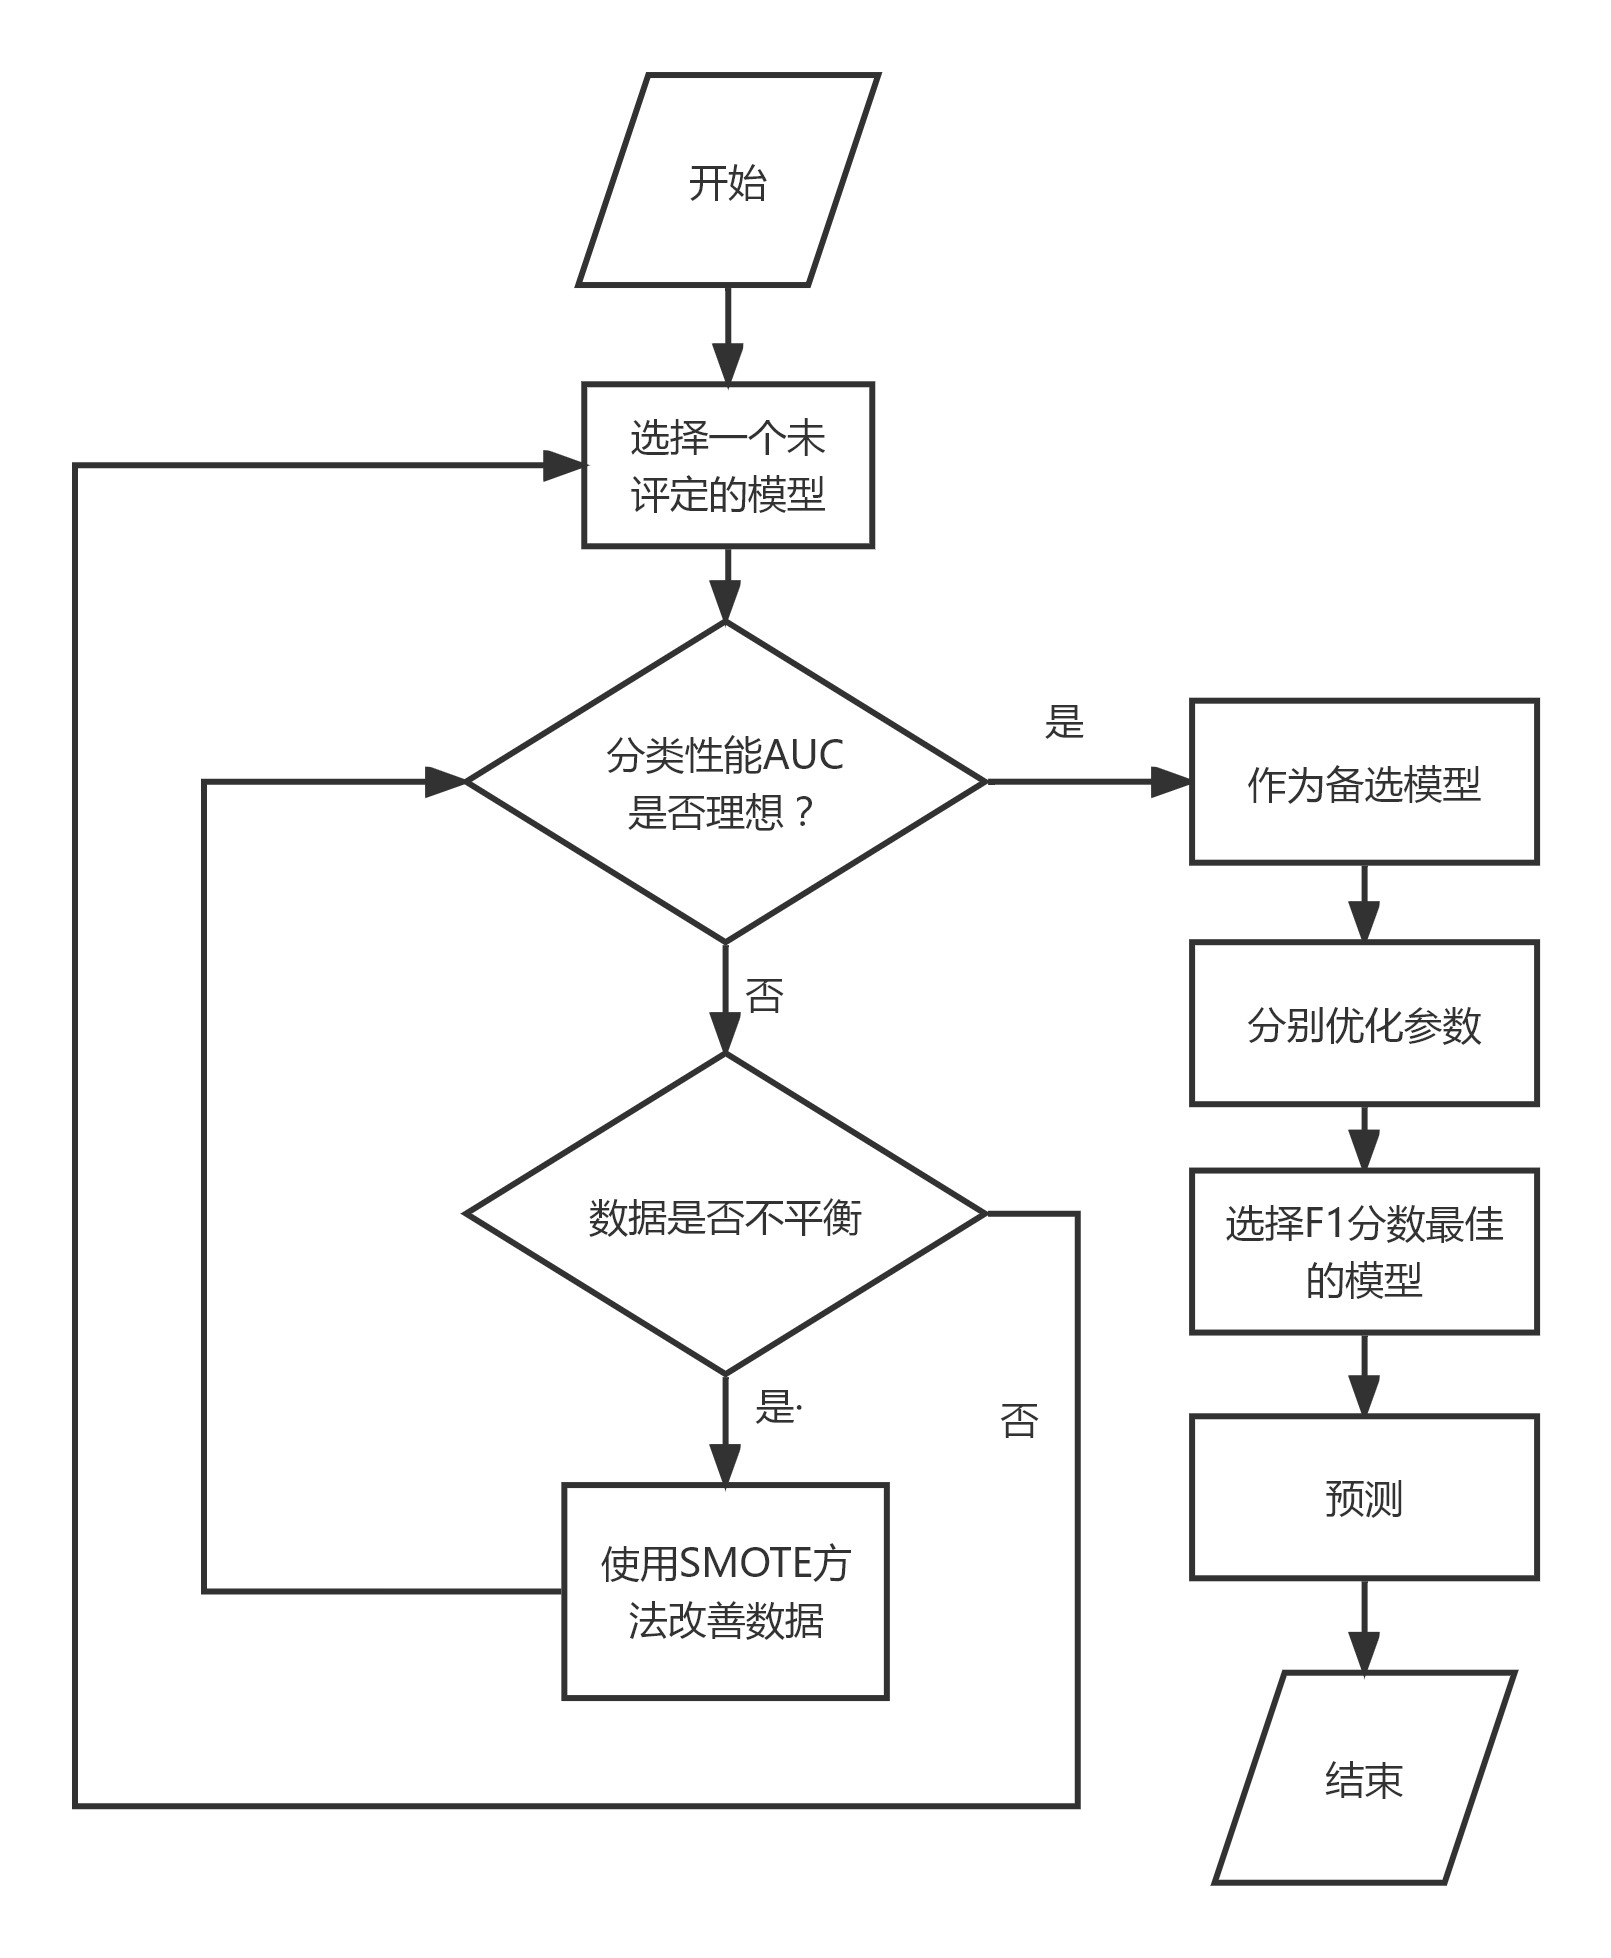
\includegraphics[width=.7\textwidth]{figures/问题1_1流程图.jpg}
\caption{血肿扩张概率预测}
\label{血肿扩张概率预测}
\end{figure}

首先是对数据集进行划分,即便题中已给出训练集,但为了评估各模型在数据集上的表现情况,仍需要对训练集进行划分,这里划分20\%的数据作为测试集,80\%的数据作为训练集,对每个模型分别进行训练,训练过程中都使用网格搜索和K折交叉验证优化模型参数,最终得到的AUC如图~\ref{采样前训练}和图~\ref{采样前测试}。

\begin{figure}
\centering
  \begin{minipage}{0.45\linewidth}
    \centering
    \includegraphics[width=\linewidth]{figures/q1_auc_train(采样前).png}
    \caption{采样前训练集}
    \label{采样前训练}
  \end{minipage}%
  \begin{minipage}{0.45\linewidth}
    \centering
    \includegraphics[width=\linewidth]{figures/q1_auc_test(采样前).png}
    \caption{采样前测试集}
    \label{采样前测试}
  \end{minipage}
\end{figure}

对于这里的任意一个模型,AUC的值都算不上优秀,所以应当反过来考虑数据本身是否有问题,还是模型选取的都不好。这里使用SMOTE方法对原始数据进行采样,使用采样后的数据对每个模型分别进行训练,训练过程中都使用网格搜索和K折交叉验证优化模型参数,最终得到的AUC如图~\ref{采样后训练}和图~\ref{采样后测试}。

\begin{figure}
\centering
  \begin{minipage}{0.45\linewidth}
    \centering
    \includegraphics[width=\linewidth]{figures/q1_auc_train(采样后).png}
    \caption{采样后训练集}
    \label{采样后训练}
  \end{minipage}%
  \begin{minipage}{0.45\linewidth}
    \centering
    \includegraphics[width=\linewidth]{figures/q1_auc_test(采样后).png}
    \caption{采样后测试集}
    \label{采样后测试}
  \end{minipage}
\end{figure}

SMOTE采样后的数据训练出来的模型AUC值都大幅提升了,结合上题对数据的探索,可以认为模型的选取是成功的,只是原始数据的分布不平衡。训练中要使用SMOTE采样解决模型性能下降的问题,使用采样后的数据训练可以避免模型倾向于预测多数样本的类别而忽略了少数样本的类别的问题。

本文选取使用模型时选择使用F1分数最大的模型,因为数据集相关的患者都是鲜活的生命,判断这种人命莜关的事件发生的概率,需要最小化误诊和漏诊的概率,只使用recall或者precision作为评价指标都有失偏颇,使用F1则可以很好的平衡这二者的关系,所以本文使用F1作为模型选取的评价指标。

\begin{table}[htbp]
    \centering
    \caption{K折交叉验证上的评价指标}
    \begin{tabular}{lccccccc}
        \hline
        模型 & AUC & ACC & Recall & Precision & F1 & CV \\
        \hline
        LR & 0.6942 & 0.6843 & 0.7900 & 0.6670 & 0.7137 & 15 \\
        RF & 0.8358 & 0.7343 & 0.7367 & 0.7492 & 0.7191 & 15 \\
        XGB & 0.8000 & 0.7102 & 0.7900 & 0.6867 & 0.7176 & 15 \\
        LGBM & 0.8135 & 0.7256 & 0.7714 & 0.7085 & 0.7306 & 10 \\
        SVC & 0.7542 & 0.7028 & 0.8300 & 0.6710 & 0.7311 & 15 \\
        MLP & 0.7591 & 0.7327 & 0.8476 & 0.6907 & 0.7533 & 10 \\
        \hline
    \end{tabular}
\end{table}

\begin{table}
\centering
\caption{是否扩张及扩张概率(仅展示部分数据)}
\label{是否扩张及扩张概率_部分表}
 \begin{spacing}{0.8}
\begin{tabular}{cccc}
\toprule
\textbf{ID} & \textbf{是否发生血肿扩张} & \textbf{血肿扩张预测概率} \\
\midrule
\textbf{sub001} & 0 & 0.0199 \\
\textbf{sub002} & 0 & 0.009 \\
\textbf{sub003} & 1 & 0.9487 \\
\textbf{sub004} & 0 & 0.0107 \\
\textbf{sub005} & 1 & 0.987 \\
\textbf{sub006} & 0 & 0.0152 \\
\textbf{sub007} & 0 & 0.014 \\
\textbf{sub008} & 1 & 0.9743 \\
\textbf{sub009} & 1 & 0.9968 \\
\textbf{sub010} & 0 & 0.0395 \\
\bottomrule
\end{tabular}
\end{spacing}
\end{table}

\subsubsection{结果分析}

观察表~\ref{是否扩张及扩张概率_部分表}(总表见附录~\ref{是否扩张及扩张概率_全表})预测的概率以及上一小节中计算的血肿扩张标签,可以看到被标记为发生血肿扩张的患者的概率值普遍大于0.5,且大多集中在0.9左右。这表明MLP模型在训练集上成功地提取了特征,准确率超过了95\%。然而,由于后60位患者的实际标记值未知,所以无法确定模型在这些患者身上的预测效果。如果后60位患者的数据分布与前100位患者的数据分布相似,那么MLP模型对于那些未知的60位患者,其预测的概率大于0.5的患者应该也是被标记的发生血肿扩张的患者。

\section{血肿周围水肿的发生及进展探索模型的建立与求解}
\subsection{模型2a的建立与求解}\label{残差计算}
\subsubsection{相关模型}\label{2种回归的章节}

\textbf{高斯拟合}\cite{Wang2018AmphibianSR}是将一组数据点拟合成高斯函数的过程。高斯函数是一个钟形曲线,也称为正态分布曲线。它由以下公式给出:

\begin{equation}
y = A \cdot e^{-\frac{(x - \mu)^2}{2\sigma^2}}
\end{equation}

\noindent 其中,$A$ 是幅值参数,控制曲线的高度;$\mu$ 是均值参数,指示曲线的中心位置;$\sigma$ 是标准差参数,决定曲线的宽度。通过拟合实际数据点到高斯函数模型,可以估计出最佳的参数值,从而得到符合数据分布的拟合曲线。

Logistic拟合是将一组二分类数据点拟合成逻辑函数的过程。逻辑函数是一种常用的 S 形曲线,也称为 Sigmoid 曲线。它由以下公式给出:

\begin{equation}
f(x) = \frac{L}{1 + e^{-k(x-x_0)}}
\end{equation}

\noindent 其中,$L$ 是饱和度参数,确定曲线的上下限;$k$ 是斜率参数,控制曲线的变化速率;$x_0$是位置参数,表示曲线的平移。通过拟合实际数据点到逻辑函数模型,可以估计出最佳的参数值,进而得到能够拟合数据的 S 形曲线。
\subsubsection{模型建立与求解}
首先从给定数据中提取前100例患者的各个检查时间点以及对应的水肿体积,将每个患者的发病时间置0,并将数据对齐,整理出所有(时间,水肿体积)元组,绘制散点图如图~\ref{数据散点图}所示。

\begin{figure}[!h]
\centering
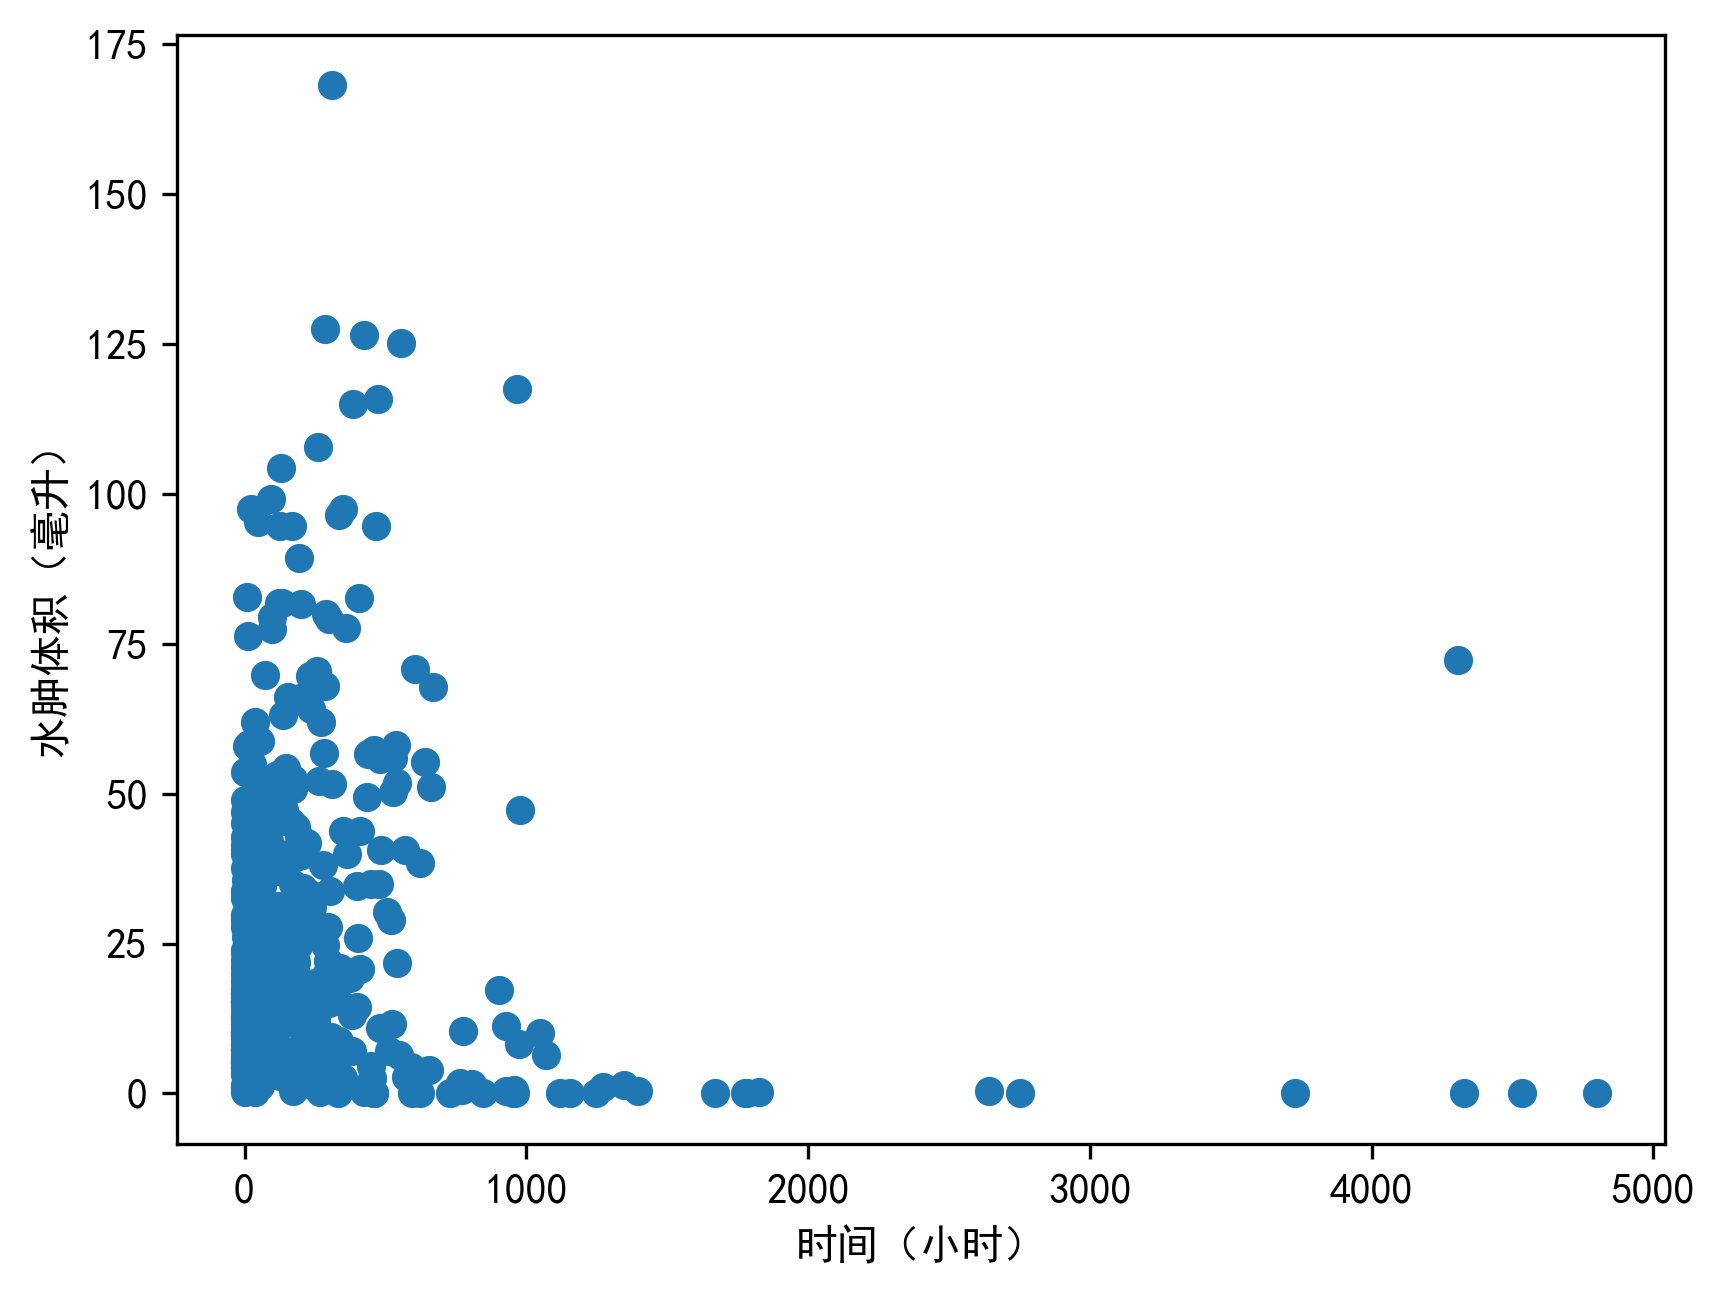
\includegraphics[width=0.8\textwidth]{fig_me/q21散点图.png}
\caption{数据散点图}
\label{数据散点图}
\end{figure}

观察图~\ref{数据散点图}可以发现,该份样本比较散乱,可能符合高斯曲线或Logistic曲线,故本节在节~\ref{6种回归的章节}的基础上增加了高斯拟合和Logistic拟合模型,继续使用本文提出的投票拟合机进行拟合,投票拟合机选取了高斯函数拟合,符合预想,得到的拟合函数如公式~\ref{高斯拟合结果}所示,拟合与散点对照图如图~\ref{拟合结果图}所示。
\begin{equation}\label{高斯拟合结果}
ED\_v(t)=40.03e^{\frac{-(t - 384.68)^2} { 2 \cdot 342.06 ^2}}
\end{equation}
\begin{figure}[!h]
\centering
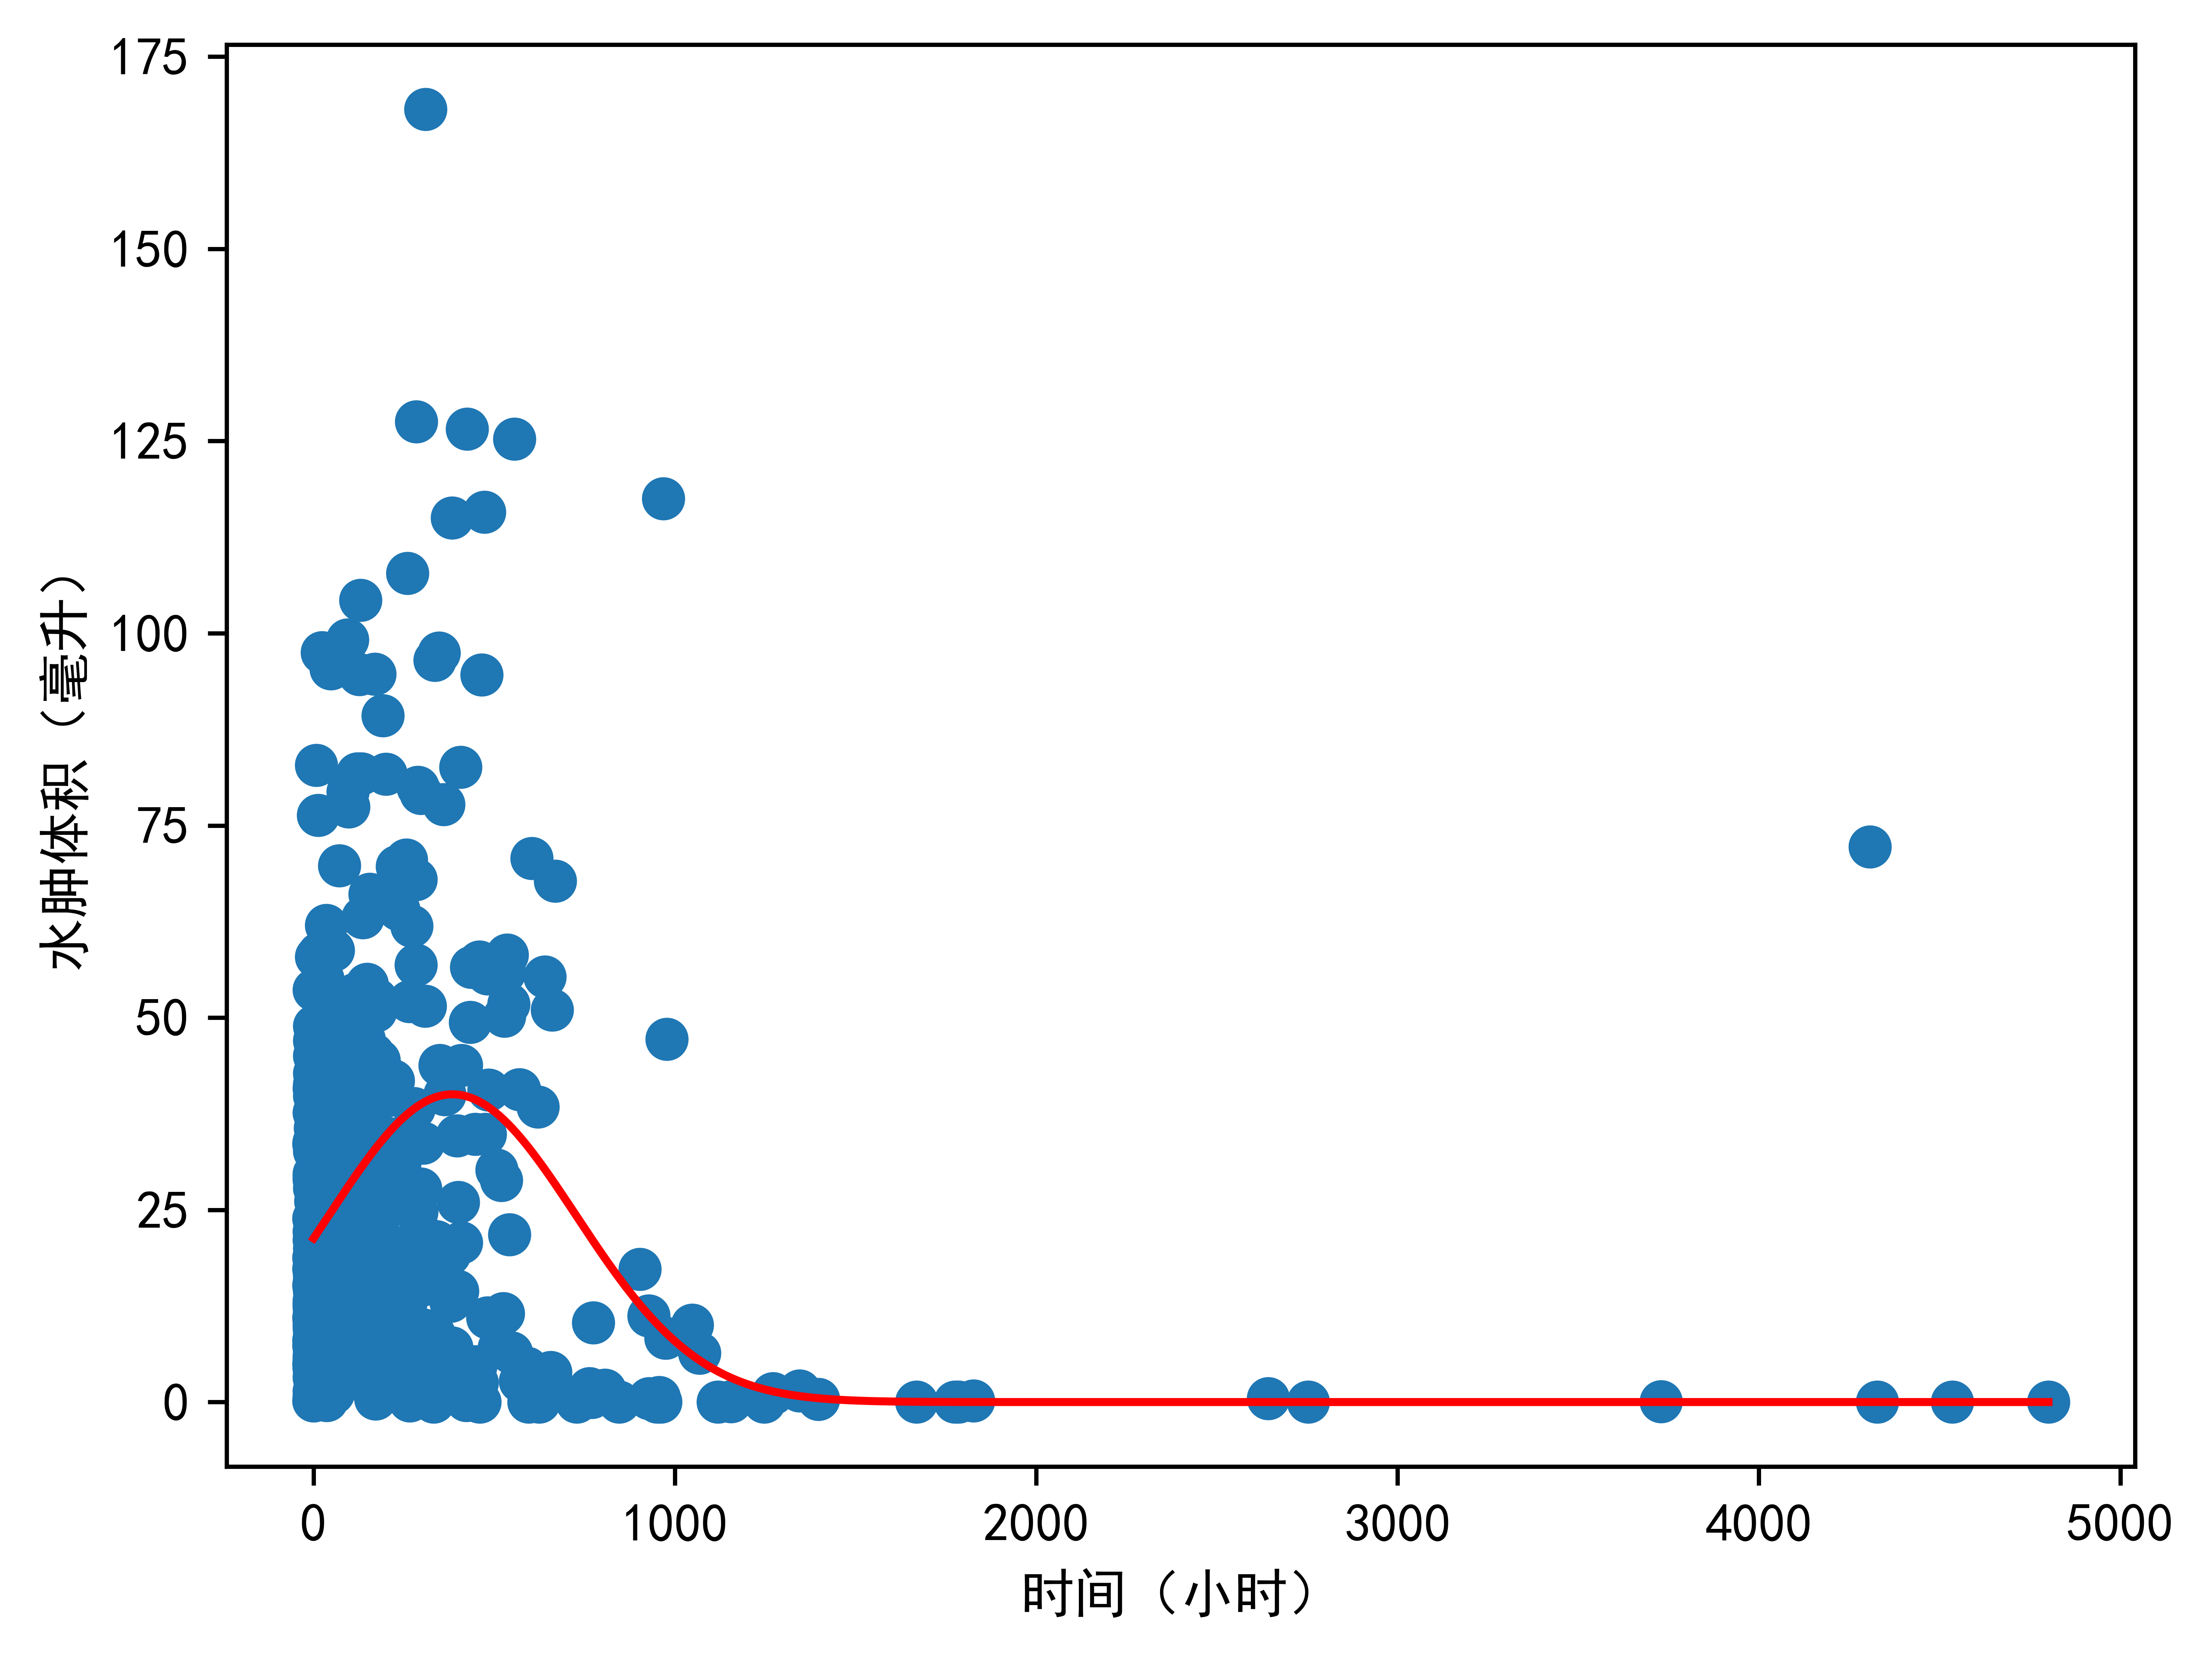
\includegraphics[width=0.8\textwidth]{fig_me/q21拟合结果图.png}
\caption{拟合结果图}
\label{拟合结果图}
\end{figure}
根据拟合结果计算出每个患者每次检查的残差,公式为公式~\ref{残差公式}

\begin{equation}\label{残差公式}
e_i = y_i-\hat{y_i}
\end{equation}

\noindent 其中,$i$代表第$i$次观测,$y_i$代表真实值,$\hat{y_i}$代表观测值。计算出每人的残差后,由于每个患者有多次检验,计算出多个残差构成个人残差列,填表结果将取每个患者的残差列的绝对值之和。结果如表~\ref{全体残差表}所示。

\begin{table}[!ht]
    \centering
    \begin{spacing}{0.7}
    \caption{全体残差表}
    \label{全体残差表}
    \begin{tabular}{cccccccc}
    \hline
        ID & 残差 & ID & 残差 & ID & 残差 & ID & 残差 \\ \hline
        sub001 & 271.9532 & sub026 & 38.9382 & sub051 & 66.2522 & sub076 & 88.8824 \\ 
        sub002 & 13.843 & sub027 & 59.897 & sub052 & 114.7003 & sub077 & 43.0182 \\ 
        sub003 & 56.2694 & sub028 & 66.8614 & sub053 & 30.4497 & sub078 & 74.0998 \\ 
        sub004 & 52.8235 & sub029 & 66.2511 & sub054 & 38.3847 & sub079 & 97.2305 \\ 
        sub005 & 41.0936 & sub030 & 190.7534 & sub055 & 35.9484 & sub080 & 50.67 \\ 
        sub006 & 228.7489 & sub031 & 40.3329 & sub056 & 155.2094 & sub081 & 151.1463 \\ 
        sub007 & 59.5779 & sub032 & 70.6233 & sub057 & 56.7305 & sub082 & 21.5298 \\ 
        sub008 & 43.4819 & sub033 & 102.8056 & sub058 & 22.979 & sub083 & 34.5179 \\ 
        sub009 & 27.0148 & sub034 & 111.3092 & sub059 & 76.274 & sub084 & 40.3026 \\ 
        sub010 & 41.795 & sub035 & 92.9648 & sub060 & 118.5478 & sub085 & 158.0197 \\ 
        sub011 & 74.6455 & sub036 & 68.3816 & sub061 & 211.1576 & sub086 & 104.2311 \\ 
        sub012 & 55.0505 & sub037 & 72.7597 & sub062 & 32.3362 & sub087 & 110.5318 \\ 
        sub013 & 94.8707 & sub038 & 42.0589 & sub063 & 235.9551 & sub088 & 12.3598 \\ 
        sub014 & 18.0059 & sub039 & 230.6566 & sub064 & 134.3079 & sub089 & 60.562 \\ 
        sub015 & 113.37 & sub040 & 116.5802 & sub065 & 70.6758 & sub090 & 109.4631 \\ 
        sub016 & 86.1556 & sub041 & 73.7108 & sub066 & 58.0217 & sub091 & 74.8485 \\ 
        sub017 & 24.761 & sub042 & 67.4386 & sub067 & 54.1227 & sub092 & 72.4169 \\ 
        sub018 & 67.6434 & sub043 & 20.2432 & sub068 & 63.5515 & sub093 & 100.0753 \\ 
        sub019 & 50.5909 & sub044 & 123.1682 & sub069 & 88.6983 & sub094 & 60.7148 \\ 
        sub020 & 90.0973 & sub045 & 33.1459 & sub070 & 48.4795 & sub095 & 359.3986 \\ 
        sub021 & 41.5674 & sub046 & 37.7441 & sub071 & 109.5165 & sub096 & 147.3067 \\ 
        sub022 & 60.7131 & sub047 & 48.2941 & sub072 & 32.4164 & sub097 & 57.7792 \\ 
        sub023 & 81.7511 & sub048 & 76.499 & sub073 & 58.106 & sub098 & 41.3645 \\ 
        sub024 & 105.0256 & sub049 & 101.761 & sub074 & 209.9081 & sub099 & 21.4809 \\ 
        sub025 & 19.7391 & sub050 & 43.8614 & sub075 & 28.3571 & sub100 & 62.881 \\ \hline
    \end{tabular}
    \end{spacing}
    
\end{table}


\subsubsection{结果分析}
根据拟合图和残差表可知,由于原始数据太过混乱,拟合效果并不佳,从数据中也患者与患者之间的总体差异较大,不能用同一条曲线表示所有患者的水肿体积随时间进展曲线,但可能存在某些子群体,他们的水肿体积随时间进展曲线可以表达为同一条曲线且效果较好。
\subsection{模型2b的建立与求解}
\subsubsection{相关模型}

上一问中的拟合曲线效果不好,这意味着患者与患者之间的总体差异较大,不能用同一条曲线表示所有患者的水肿体积随时间进展曲线,但可能存在某些子群体,他们的水肿体积随时间进展曲线可以表达为同一条曲线且效果较好,这里使用以下几个算法探讨对患者的分组情况,再分别进行曲线拟合。

\textbf{K-Means(K均值聚类)}\cite{emon2020performance}是一种迭代聚类算法,用于将数据集分成K个不重叠的簇(群组)。该算法随机选择K个簇中心点,然后将数据点分配给最近的簇中心,接着更新簇中心,重复这个过程直到收敛。K均值聚类以最小化簇内数据点的方差作为优化目标,因此适用于发现紧密聚集的簇。

\textbf{Hierarchical Clustering(层次聚类)}\cite{zihni2020opening}是一种基于树状结构的聚类方法,它将数据点逐渐合并成更大的簇,直到形成一个包含所有数据点的单一簇。这个层次结构可以表示为树状图,其中每个节点代表一个簇,从根节点开始,通过逐步合并子簇来构建整个聚类层次。层次聚类可用于识别不同层次的聚类结构,从细粒度到粗粒度。

\textbf{Birch(平衡迭代规约和聚类)}\cite{guha2003clustering}是一种聚类算法,旨在高效处理大规模数据集。它采用一种层次化的聚类方法,首先通过构建一个紧凑的数据结构(CF树)来降低内存占用和计算复杂度,然后对CF树进行聚类。Birch在处理高维数据和大型数据集时表现出色,能够找到具有不同形状和大小的簇。

\textbf{Spectral Clustering(谱聚类)}\cite{razzak2020big}是一种基于数据点之间的相似性矩阵的聚类方法。它将数据点视为图的节点,并根据它们之间的相似性构建图的邻接矩阵。然后,通过分析该邻接矩阵的特征向量来划分数据点。谱聚类适用于发现不规则形状的簇,特别适合处理图像分割和社交网络分析等应用。

各模型聚类分组的效果用以下两个评价指标做评价:

\textbf{Silhouette coefficient(Silhouette系数)}是一种用于度量数据点聚类紧密度的指标。它通过计算每个数据点与其所属簇内其他数据点的相似性以及与最近簇中的数据点的不相似性来评估聚类的有效性。Silhouette系数的取值范围在-1到1之间,其中高于0的值表示数据点被正确聚类,而接近0的值表示数据点位于簇的边界附近,而负值则表示数据点可能被错误聚类。

\textbf{Calinski-Harabasz index(Calinski-Harabasz指数)}是一种用于衡量聚类分离度的指标。它通过计算簇内数据点的方差与簇间数据点的方差之比来评估聚类的紧密性和分离度。具体而言,较高的Calinski-Harabasz指数表示簇内数据点之间的方差较小,而簇之间的方差较大,这通常对于更好的聚类结果是有益的。因此,该指数可用于比较不同聚类算法或不同聚类数目的聚类结果。

\subsubsection{模型建立}

原始数据包含性别、年龄、每个检测时间点的水肿体积大小,对年龄进行one-hot编码后,还需要使用z-score归一化所有数据,避免有些特征数值大导致算法运行过程中被给与了更高的权重。题设中要求分组在3~5组,所以先对每个模型使用默认参数,聚类中心设置3、4、5分别求解,得到下表的评价指标:

\begin{table}[ht]
\centering
\caption{聚类性能评估}
\begin{tabular}{cccccccc}
\toprule
\multirow{2}{*}{\textbf{评估指标}} & \multirow{2}{*}{\textbf{聚类中心数}}& \multicolumn{4}{c}{\textbf{聚类方法}}  \\
\cmidrule{3-6}
&& \textbf{K-Means} & \textbf{Hierarchical} & \textbf{Birch} & \textbf{Spectral} \\
\midrule
\multirow{2}{*}{\textbf{Silhouette coefficient}}&3 & 0.6016 & 0.5932 & 0.5499 & 0.5266  \\
& 4& 0.6307 & 0.6365 & 0.5426 & 0.6190  \\
& 5& 0.6890 & 0.6870 & 0.5926 & 0.6870  \\
\midrule
\multirow{2}{*}{\textbf{Calinski-Harabasz}} & 3& 51.6382 & 46.6169 & 36.6422 & 29.1885  \\
& 4& 48.7829 & 47.1112 & 27.0804 & 42.7551  \\
& 5& 48.8069 & 49.7575 & 32.1278 & 48.8459  \\
\bottomrule
\end{tabular}
\end{table}

从评价指标中不难看出K均值聚类的Silhouette系数在所有可能的聚类中心的分组中都是最大的,所以本文选用K均值聚类对患者进行分组。

\subsubsection{模型求解}

使用默认参数的K均值聚类仍然有很大的优化空间,这里使用网格搜索进行超参数选取,最终选择的超参数值分别为:初始化聚类中心使用“k-means++”方法, 最大迭代次数1次, 聚类中心为5个,最终得到的Silhouette系数为0.69,Calinski-Harabasz指数是50.56。根据分组结果,使用在节~\ref{6种回归的章节}和节~\ref{2种回归的章节}提到的8种回归算法,进行五组回归,并使用节~\ref{残差计算}中的方法计算分组后前100名患者的残差,结果如表~\ref{分组残差表}所示。


\subsubsection{结果分析}
\begin{figure}[!h]
\centering
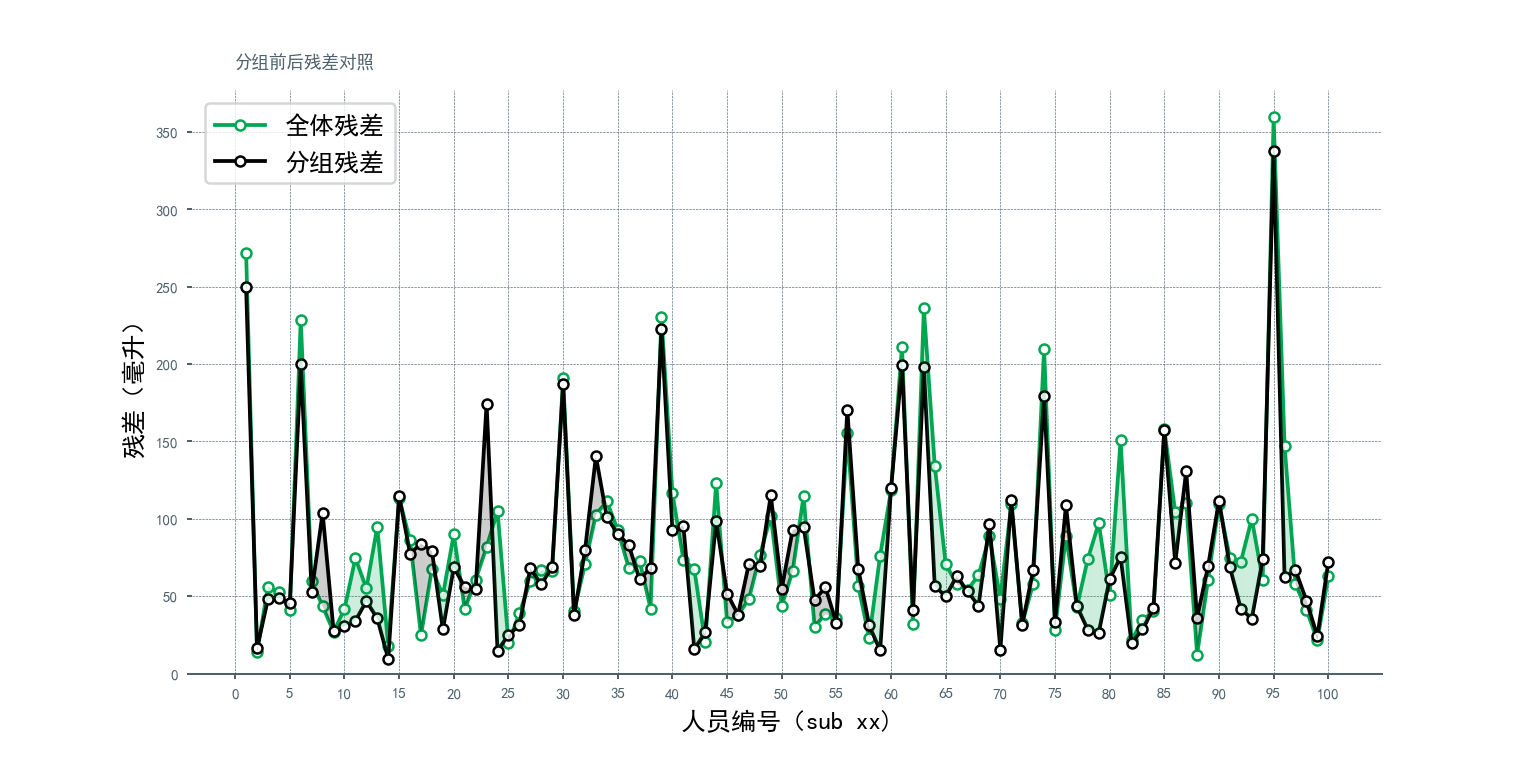
\includegraphics[width=\textwidth]{fig_me/残差对照.png}
\caption{分组前后残差对照}
\label{分组前后残差对照}
\end{figure}

\begin{figure}[!h]
\centering
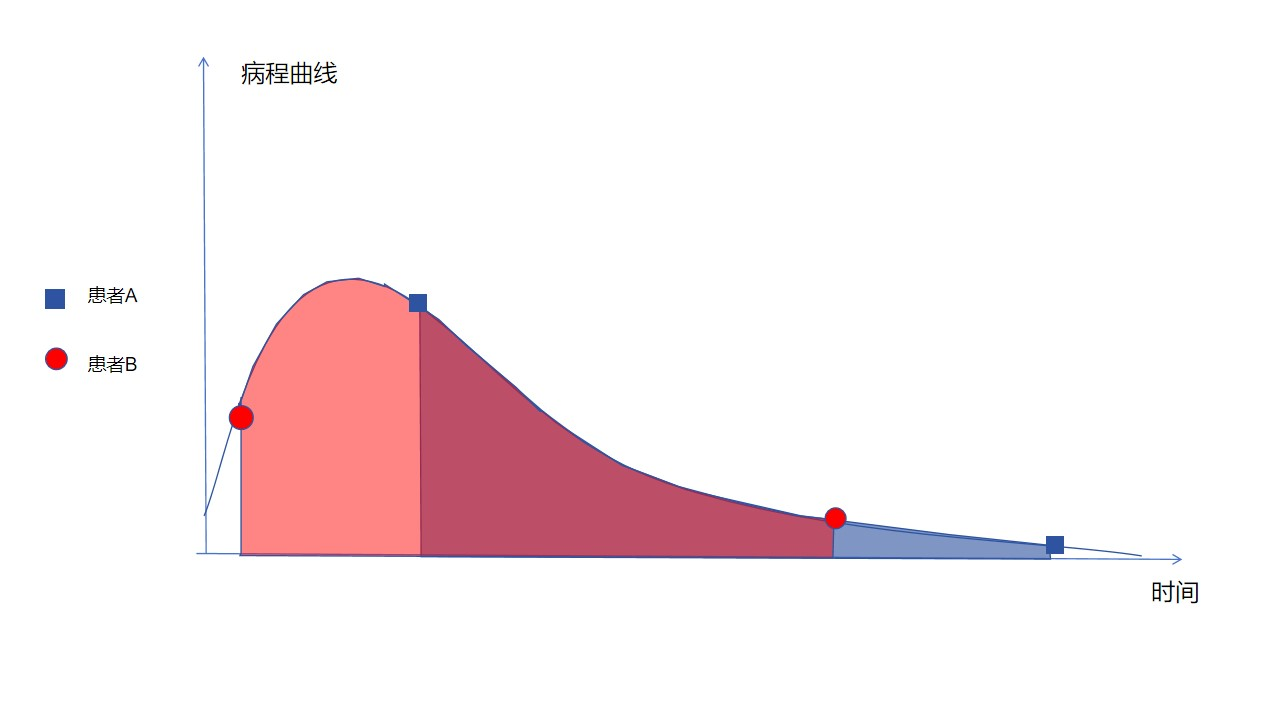
\includegraphics[width=.7\textwidth]{figures/病程曲线.jpg}
\caption{病程曲线图}
\label{病程曲线}
\end{figure}

经过分组后,总体残差下降,如图~\ref{分组前后残差对照}所示,说明分组取得一定的出成效,但是由于组间个体差异依旧较大,对分组后的患者数据进行拟合,并未取得理想的效果,然而这并非偶然现象。这一情况存在其合理原因:每个患者都有一个病程曲线,假设每位患者的病程曲线大致呈现相似的趋势,即在患者生病后,病情逐渐上升,然后在治愈过程中下降。然而,不同患者之间仍可能存在病情波动的幅度差异,即病情最为严重的程度可能存在差异。另一方面,即便假设各患者的病程曲线趋势大致相似,即病情最为严重的程度相似,仍然有一个关键差异点,那就是患者就医的时间点,如图~\ref{病程曲线}。不同患者在病程曲线上就医的时间点各不相同,这也导致了后续病情发展的不同趋势。有些患者可能在就医后继续经历病情上升,然后下降,而有些患者可能在就医后病情直接开始下降。因此,在同一时间段内的医院记录的患者数据上进行拟合,实际上相当于将每个患者在就医时间点后的病程曲线合并在一起,而同一时刻的个体之间存在显著差异,这是导致拟合曲线残差较大的主要原因之一。


\subsection{模型2c的建立与求解}

\subsubsection{相关模型}

\textbf{多元广义线性模型(GLM)}\cite{GLM}是一种在统计学和数据分析领域广泛应用的模型,其旨在建立因变量与一个或多个自变量之间的关系。GLM不仅适用于连续型因变量,还可以处理二元、多元分类以及计数数据等不同类型的响应变量。该模型的核心思想是通过链接函数将自变量与因变量之间的关系进行建模,并使用指数族分布来描述因变量的分布特性。

\subsubsection{模型建立}

上一小节将全体患者分为5个亚组后,为每个患者赋予模式编号。鉴于每位患者的水肿体积特征具有不同的数值尺度,本文首先对数据进行标准化。在标准化数据的基础上,为了分析医疗干预方法对水肿体积进展模式的影响,本文使用多元广义线性模型(GLM)对数据进行拟合。其中,GLM公式如下:

\begin{equation}
g(\mu) = X\beta
\end{equation}

\noindent 其中:
$g(\mu)$ 是连接函数(Link Function),用于将线性预测值 $\mu$ 转换为非负的预测值,$X$ 是设计矩阵(Design Matrix),包含了自变量的观测值$\beta$ 是参数向量,包含了模型的系数,$\mu$ 是响应变量的均值。

\subsubsection{模型求解}

需要先总结已有的治疗方法,统计后如表~\ref{组合治疗分组对照表}。将治疗方法分为两类来分析,一类是组合治疗方法,一共有28组;一类是单一治疗方法,一共有7种。分别将单一治疗方法,治疗方法组合作为解释变量,得到的回归结果为表~\ref{单一治疗方法和治疗方法组合的统计数据}、表~\ref{单一治疗方法的回归系数及显著性}和表~\ref{组合治疗方法的回归系数及显著性}(见附录)。

\begin{table}[htbp]
\centering
\caption{单一治疗方法和组合治疗方法的统计数据}
\label{单一治疗方法和治疗方法组合的统计数据}
\begin{tabular}{lccc}
\toprule
& 单一治疗方法 & 治疗方法组合 \\
\midrule
F-statistic & 1.132 & 0.9185 \\
Prob (F-statistic) & 0.350 & 0.555 \\
Log-Likelihood & -137.76 & -133.18 \\
AIC & 291.5 & 302.4 \\
Df Residuals & 92 & 82 \\
BIC & 312.4 & 349.2 \\
Durbin-Watson & 2.327 & 2.396 \\
Jarque-Bera (JB) & 13.012 & 12.210 \\
Skew & -0.090 & -0.005 \\
Kurtosis & 1.242 & 1.288 \\
\bottomrule
\end{tabular}
\end{table}

\begin{table}[htbp]
  \centering
  \caption{单一治疗方法的回归系数及显著性}
   \label{单一治疗方法的回归系数及显著性}
    \begin{tabular}{lcccccc}
    \toprule
    变量 & coef & std err & t & P$>|t|$ & [0.025 & 0.975] \\
    \midrule
    const & -0.2209 & 0.768 & -0.288 & 0.774 & -1.745 & 1.304 \\
    脑室引流 & -0.0630 & 0.426 & -0.148 & 0.883 & -0.910 & 0.784 \\
    止血治疗 & -0.4166 & 0.285 & -1.461 & 0.147 & -0.983 & 0.150 \\
    降颅压治疗 & 0.3487 & 0.278 & 1.255 & 0.213 & -0.203 & 0.901 \\
    降压治疗 & 0.7816 & 0.410 & 1.906 & 0.060 & -0.033 & 1.596 \\
    镇静、镇痛治疗 & 0.1893 & 0.317 & 0.598 & 0.551 & -0.439 & 0.818 \\
    止吐护胃 & -0.5453 & 0.678 & -0.804 & 0.423 & -1.892 & 0.801 \\
    营养神经 & -0.0648 & 0.538 & -0.120 & 0.904 & -1.134 & 1.004 \\
    \bottomrule
    \end{tabular}%
\end{table}%

\subsubsection{结果分析}

观察表~\ref{单一治疗方法和治疗方法组合的统计数据}、表~\ref{单一治疗方法的回归系数及显著性}和表~\ref{组合治疗方法的回归系数及显著性},可以发现降压治疗在单一治疗方法作为解释变量时呈现出了接近显著性水平的P值(0.060),这提示着降压治疗可能对目标变量具有某种程度的影响。然而,当考虑了治疗方法的组合时,本文观察到了一个有趣的现象,即治疗组合7(P值为0.115)显示出相对较低的显著性水平。这似乎表明治疗组合7可能对目标变量具有一定的显著影响,但必须注意的是,研究中存在多重共线性关系,即一些治疗方法组合依赖于其他组合的情况。这种情况可能导致交互效应的存在,即不同治疗方法之间可能存在相互作用,而这些相互作用可能影响了观察到的显著性水平。此外,这里也要考虑因果关系,即治疗方法是否直接导致了目标变量的变化,或者是否存在其他潜在的因果途径。最后,治疗路径的依赖性也是一个需要关注的因素,不同的治疗方法组合可能导致不同的治疗路径,这可能影响了治疗效果的解释和预测。

\subsection{模型2d的建立与求解}

\subsubsection{相关模型}

\textbf{方差分析}\cite{ANOVA}是一种统计方法,用于比较三个或更多组之间的均值差异。它通常用于确定一个或多个因变量如何受一个或多个自变量的影响,以及这些影响是否显著。方差分析的主要思想是将总方差分解为组内方差和组间方差,然后通过比较这两种方差来确定组别之间是否存在显著差异。

在方差分析中,首先收集数据,将观测值分成不同的组别,然后计算每个组的均值和方差。接下来,使用统计测试来比较这些组的均值,以确定它们之间是否存在显著差异。这里将使用该方法探讨各治疗方法(自变量)对患者水肿体积进展模式(因变量)的影响。

\subsubsection{模型建立与求解}

对于血肿体积、水肿体积及治疗方法这三者之间的关系分析,这里选择将它们两两一起分析,当分析治疗方法对血肿体积和水肿体积的影响时,使用方差分析方法进行分析;当分析血肿体积和水肿体积之间的关系时,通过使用本文提出的投票拟合机,选出了拟合的模型,使用线性回归模型进行拟合。

本文进行单因素方差分析(One-Way ANOVA)来比较治疗方法对五个患者群的影响。方差分析将生成F统计量和p值,用于检验组间均值的差异是否显著。F统计量和P值计算公式如式~\ref{F值}、式~\ref{P值}。

\begin{equation}
F = \frac{MS_{\text{between}}}{MS_{\text{within}}}
\label{F值}
\end{equation}

\begin{equation}
p = P(F \geq F_{\text{observed}} | df_{\text{between}}, df_{\text{within}})
\label{P值}
\end{equation}

\noindent 其中,$F$代表F统计量,$MS_{\text{between}}$代表组间均方差,$MS_{\text{within}}$代表组内均方差,$F_{\text{observed}}$代表观察到的F统计量值,$df_{\text{between}}$代表组间自由度,$df_{\text{within}}$代表组内自由度。

由于上一小节有提取出治疗方法中的单一和组合两大类型,所以这里的治疗方法也沿用上一小节的定义,血肿和水肿的数据则需要进行处理,使用后一次检测的体积大小减去前一次检测的体积大小,如果差值为正则累加1,否则累加-1,最后该患者的血肿/水肿体积变动累加值即为他个人的体积变动趋势。血肿/水肿的体积变动趋势分别作为因变量,所有治疗方法一一作为自变量,进行方差分析,结果如表~\ref{单一治疗方法与血肿、水肿之间的P值和F值}和表~\ref{组合治疗方法与血肿、水肿之间的P值和F值},组合治疗的分组对照表~\ref{组合治疗分组对照表}(见附录)。

\begin{table}[h]  % 显示位置为当前位置
	\centering     % 显示位置为中间
	\caption{单一治疗方法与血肿、水肿之间的P值和F值}  % 表格题目
	\label{单一治疗方法与血肿、水肿之间的P值和F值}        % 引用标签
	\begin{tabular}{ c c c c c }  % 5列
		\toprule[1.5pt]   % 上边线(或表示为)
		
		% 合并单元格
		\multirow{2}{1cm}{治疗方法} & \multicolumn{2}{c}{水肿} & \multicolumn{2}{c}{血肿} \\ 
						&P-value    & F-value  & P-value    & F-value   \\ 
		
		\midrule[1pt]     % 中线(或表示为)
		
		脑室引流	 	& 1       & 0      & \textbf{0.1292 }&\textbf{ 2.3413} \\ 
		止血治疗		& 0.8084  & 0.0591 & 0.3589 & 0.8497 \\ 
		降颅压治疗	    & \textbf{0.1633}  & \textbf{1.9732} & \textbf{0.1943} & \textbf{1.7083} \\ 
		降压治疗 		& \textbf{0.027}   &\textbf{ 5.04}   & 0.9655 & 0.0019 \\ 
		镇静、镇痛治疗 	& 0.7821  & 0.0769 & 0.387  & 0.755  \\ 
            止吐护胃 		& 0.5624  & 0.3379 & 0.2924 & 1.1206 \\ 
            营养神经 		& 1       & 0      & 0.4352 & 0.614  \\ 
		
		\bottomrule[1.5pt]   % 下边线(或表示为)
	\end{tabular} 
\end{table}



\begin{table}[h]  % 显示位置为当前位置
	\centering     % 显示位置为中间
	\caption{组合治疗方法与血肿、水肿之间的P值和F值}  % 表格题目
	\label{组合治疗方法与血肿、水肿之间的P值和F值}        % 引用标签
	\begin{tabular}{ c c c c c ccccc}  % 5列
		\toprule[1.5pt]   % 上边线(或表示为)
		
		% 合并单元格
		\multirow{2}{1cm}{治疗组合} & \multicolumn{2}{c}{水肿} & \multicolumn{2}{c}{血肿}&\multirow{2}{1cm}{治疗组合} & \multicolumn{2}{c}{水肿} & \multicolumn{2}{c}{血肿}  \\ 
		&P-value    & F-value  & P-value    & F-value&	&P-value    & F-value  & P-value    & F-value   \\ 
		
		\midrule[1pt]     % 中线(或表示为)
		
        1 & 0.4048  & 0.7000  & 0.7856  & 0.0744& 15 & 1.0000  & 0.0000  & \textbf{0.1292}  & \textbf{2.3413}  \\
        2 & \textbf{0.0693}  & \textbf{3.3720}  & 0.0771  & 3.1921&  16 & \textbf{0.1941}  & \textbf{1.7093}  & \textbf{0.1764}  & \textbf{1.8541}  \\
        3 & 0.6436  & 0.2154  & 0.1943  & 1.7083&  17 & 0.3392  & 0.9224  & 0.9210  & 0.0099  \\
        4 & 0.4036  & 0.7038  & 0.1074  & 2.6395&  18 & 0.4098  & 0.6853  & \textbf{0.1537 } & \textbf{2.0669}  \\
        5 & 0.6524  & 0.2042  & 0.2767  & 1.1963&  19 & 1.0000  & 0.0000  & \textbf{0.1205}  & \textbf{2.4538}  \\
        6 & 0.6719  & 0.1805  & 0.0715  & 3.3206&   20 & 0.5391  & 0.3798  & 0.1809  & 1.8159  \\
        7 & \textbf{0.0761}  & \textbf{3.2131}  & 0.1205  & 2.4538&  21 & 0.6766  & 0.1750  & \textbf{0.1074}  & \textbf{2.6395}  \\
        8 & 0.7926  & 0.0695  & 0.5365  & 0.3848& 22 & 0.3142  & 1.0234  & \textbf{0.1086}  & \textbf{2.6219}  \\
        9 & 0.3775  & 0.7861  & 0.7866  & 0.0737&  23 & 0.3052  & 1.0624  & \textbf{0.1809}  &\textbf{ 1.8159}  \\
        10 & 0.6524  & 0.2042  & 0.2767  & 1.1963& 24 & 0.6503  & 0.2068  & \textbf{0.0666}  & \textbf{3.4413}  \\
        11 & 0.3781  & 0.7840  & 0.3728  & 0.8015&  25 & 1.0000  & 0.0000  & 0.4714  & 0.5227  \\
        12 & 0.6766  & 0.1750  & 0.3262  & 0.9735& 26 & 0.4228  & 0.6479  & \textbf{0.1285}  & \textbf{2.3499}  \\
        13 & \textbf{0.1254}  & \textbf{2.3891}  & 0.1469  & 2.1384&  27 & 1.0000  & 0.0000  & 0.4714  & 0.5227  \\
        14 & 0.8360  & 0.0431  & 0.3711  & 0.8074&  28 & 1.0000  & 0.0000  & 0.4714  & 0.5227 \\
		\bottomrule[1.5pt]   % 下边线(或表示为)
	\end{tabular} 
\end{table}

血肿与水肿体积回归的二次函数曲线如图~\ref{血肿水肿关系全局拟合图}所示,为了显示出图形特征,截取图像右上角如图~\ref{血肿水肿局部拟合图}所示。

\begin{figure}[!h]
\centering
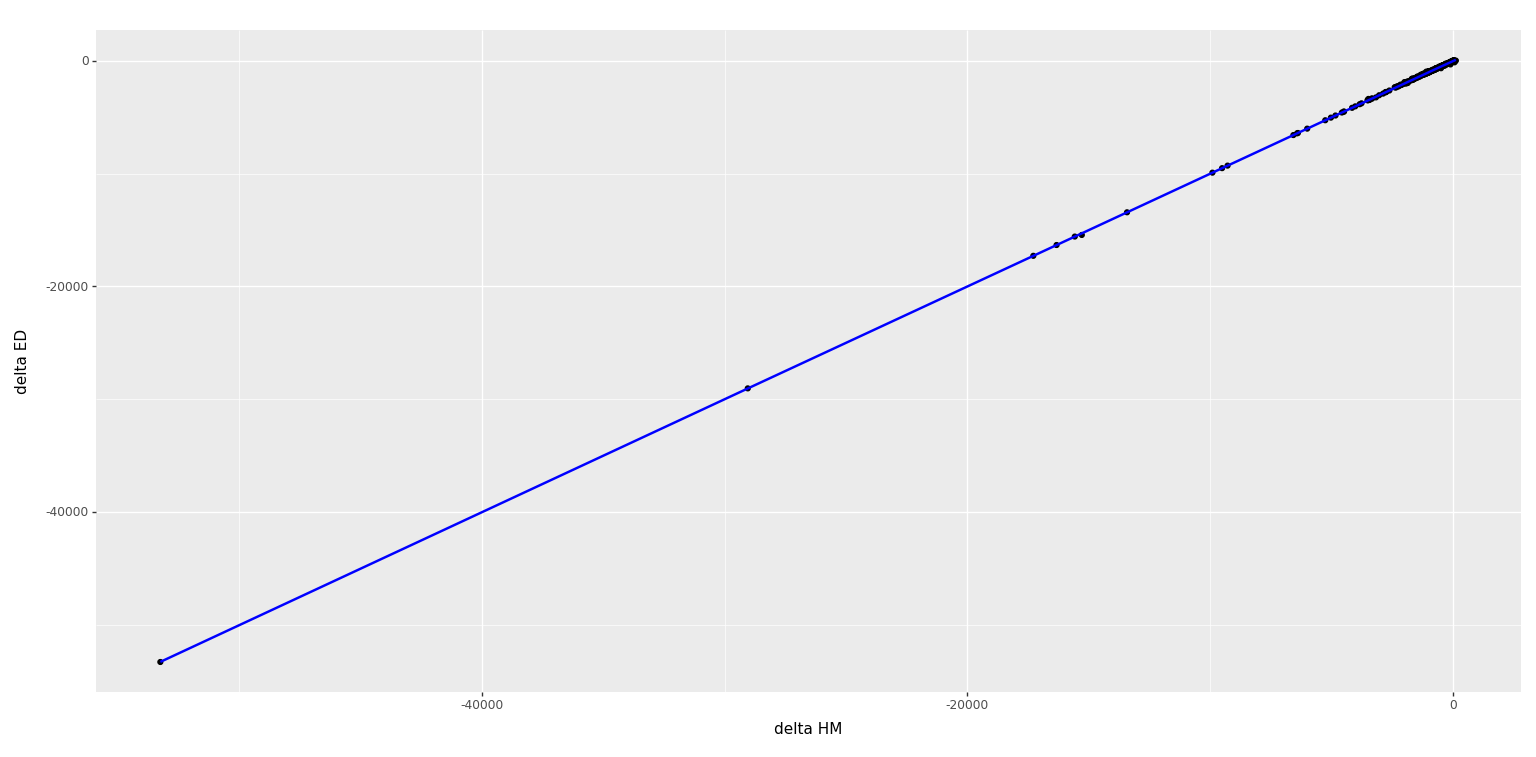
\includegraphics[width=\textwidth]{fig_me/血肿水肿关系全局拟合图.png}
\caption{血肿水肿关系全局拟合图}
\label{血肿水肿关系全局拟合图}
\end{figure}

\begin{figure}[!h]
\centering
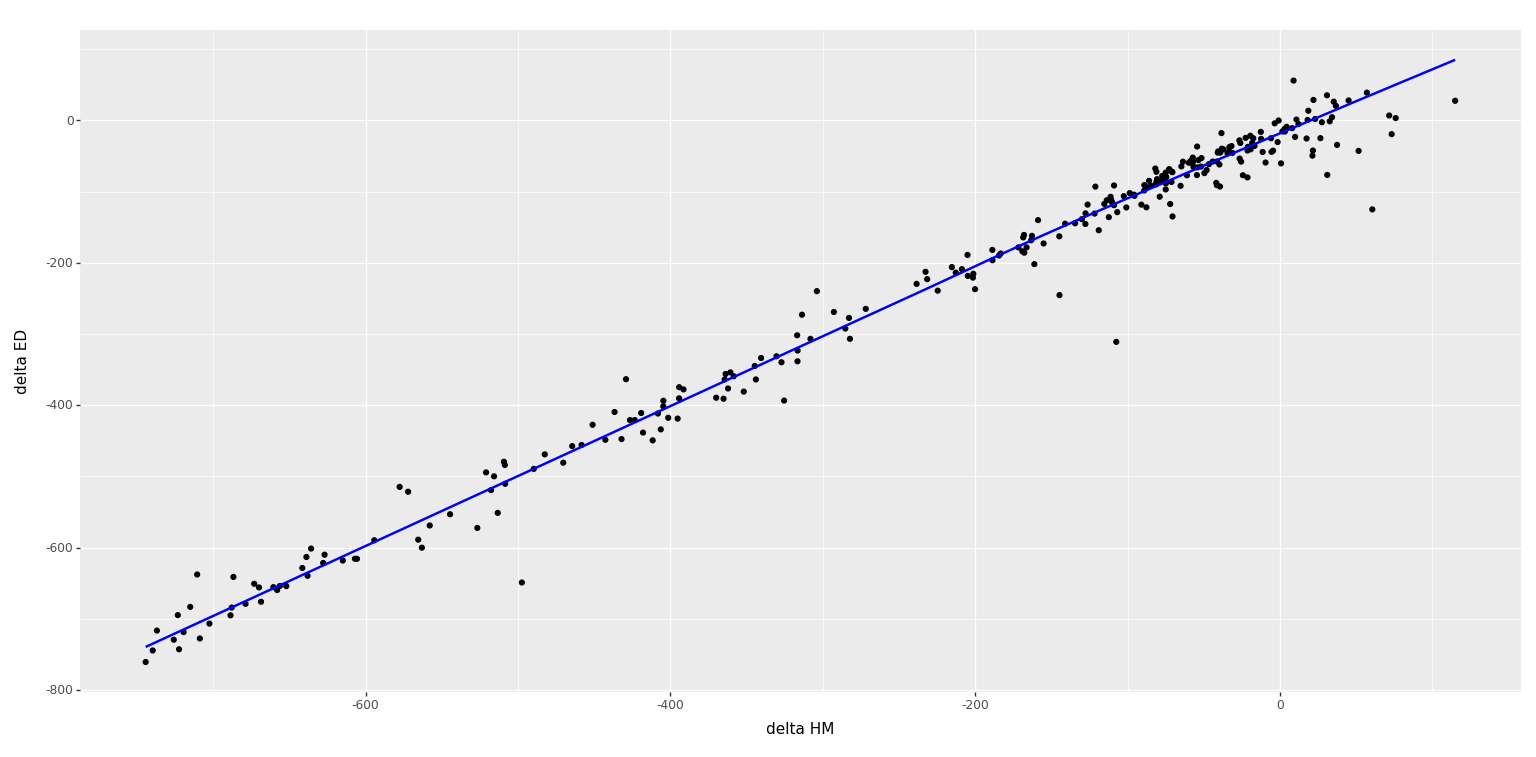
\includegraphics[width=\textwidth]{fig_me/血肿水肿局部拟合图.png}
\caption{血肿水肿局部拟合图}
\label{血肿水肿局部拟合图}
\end{figure}

\subsubsection{结果分析}

通过观察表~\ref{单一治疗方法与血肿、水肿之间的P值和F值}和表~\ref{组合治疗方法与血肿、水肿之间的P值和F值}可以发现,如果只探讨单一治疗方法,那么降颅压治疗对水肿和血肿扩张的治疗效果都显著,脑室引流只对血肿扩张的治疗效果显著,降压治疗只对水肿扩张的治疗效果显著;如果只探讨组合治疗方法,那么治疗组合2、7、13只对水肿扩张的治疗效果显著,治疗组合15、18、19、21、22、23、24、26只对血肿扩张的治疗效果显著,而治疗组合16对水肿和血肿扩张的治疗效果都显著。通过分析它们之间的依赖关系,可以发现降压治疗和降颅压治疗都是这些效果显著的治疗组合中最常见的单一治疗方法,所以综合来看,降颅压治疗是效果最好的单一治疗方法,治疗组合16则是效果最好的治疗组合。

通过观察图~\ref{血肿水肿关系全局拟合图},可以发现血肿和水肿大致呈现二次函数大致呈现二次函数形式,其拟合出的函数式如式~\ref{血肿水肿拟合曲线},检测含局部点特征的图~\ref{血肿水肿局部拟合图},可以发现拟合效果良好,血肿和水肿的体积大小大多同升同降,呈正线性相关趋势。

\begin{equation}
y = x - 0.79
\label{血肿水肿拟合曲线}
\end{equation}

\section{出血性脑卒中患者预后预测模型的建立与求解}
\subsection{模型3a的建立与求解}
\subsubsection{相关模型}


\textbf{BP神经网络},或反向传播神经网络(Backpropagation Neural Network)\cite{BP},是一种多层前馈神经网络,通常由输入层、隐含层(可以有一层或多层),和输出层组成。BP神经网络的学习过程包括两个主要阶段:前向传播和误差反向传播。

前向传播的相关流程如下:

1. 对于输入层到隐含层的神经元(每个隐含层神经元$j$):
\begin{equation}
z_j = \sum_{i=1}^{n} (x_i \cdot w_{ij}^{(ih)}) + b_j^{(h)} \\
y_j = \frac{1}{1 + e^{-z_j}}
\end{equation}

\noindent 其中,$x_i$ 是输入层的输入信号,$w_{ij}^{(ih)}$ 是输入层到隐含层神经元$j$的连接权重,$b_j^{(h)}$ 是隐含层神经元$j$的偏置,$n$ 是输入层的神经元数量,$e$ 是自然对数的底。

2. 对于隐含层到输出层的神经元(每个输出层神经元$k$):
\begin{equation}
z_k = \sum_{j=1}^{m} (y_j \cdot w_{jk}^{(ho)}) + b_k^{(o)} \\
o_k = \frac{1}{1 + e^{-z_k}}
\end{equation}

\noindent 其中,$y_j$ 是隐含层的输出信号,$w_{jk}^{(ho)}$ 是隐含层到输出层神经元$k$的连接权重,$b_k^{(o)}$ 是输出层神经元$k$的偏置,$m$ 是隐含层的神经元数量。

3. 最终的输出信号为$o_k$,它表示了神经网络的预测或分类结果。

以下是误差反向传播的相关流程:

1. 计算输出层神经元的误差信号:

\begin{equation}
\frac{\partial E}{\partial z_j} = \frac{\partial E}{\partial y_j} \cdot \frac{\partial y_j}{\partial z_j} = -(t_j - o_j) \cdot f'(z_j)
\end{equation}

\noindent 其中:$E$ 表示总误差,$z_j$ 表示输出层神经元的总输入,$y_j$ 表示输出层神经元的输出,$t_j$ 表示期望输出,$o_j$ 表示实际输出,$f'(z_j)$ 表示激活函数的导数。

2. 计算隐含层神经元的误差信号:

\begin{equation}
\frac{\partial E}{\partial z_h} = \sum_{j} \left( \frac{\partial E}{\partial z_j} \cdot \frac{\partial z_j}{\partial y_h} \cdot \frac{\partial y_h}{\partial z_h} \right)
\end{equation}

\noindent 其中:$z_h$ 表示隐含层神经元的总输入,$y_h$ 表示隐含层神经元的输出。

3. 更新输出层到隐含层的连接权重:

\begin{equation}
\Delta w_{ih} = -\alpha \cdot \frac{\partial E}{\partial w_{ih}}
\end{equation}

\noindent 其中:$\alpha$ 表示学习率,$\Delta w_{ih}$ 表示连接权重的更新量。

4. 更新输入层到隐含层的连接权重:

\begin{equation}
\Delta w_{ji} = -\alpha \cdot \frac{\partial E}{\partial w_{ji}}
\end{equation}

\noindent 其中,$\Delta w_{ji}$ 表示连接权重的更新量。

这些公式组成了误差反向传播算法的核心,通过反复迭代更新权重和阈值,神经网络可以逐渐优化其性能,使误差最小化。





\subsubsection{模型建立}\label{IACO-BP}

根据前100个患者的个人史、疾病史、发病相关,首次影像结果以及mRS评分构建BP神经网络用于预测160个患者的mRS评分时,往往会遇到以下这些问题,本文尝试用蚁群算法(ant colony algorithm)\cite{ACO}分别解决:

数据不足:数据不足导致模型的泛化能力不足。而蚁群算法可以帮助改善BP神经网络的泛化能力,尤其是当数据有限时,通过蚁群算法可以优化BP神经网络的权值,以提高模型性能。

模型复杂度:BP神经网络的复杂度取决于其结构和参数设置。如果网络结构过于简单或过于复杂,都可能导致模型的性能下降。而蚁群算法通常用于解决组合优化问题,可以帮助确定神经网络的阈值参数。

因此,在BP神经网络的基础上,本文使用基于蚁群算法的BP神经网络来建立模型。对于蚂蚁群算法,信息素的更新起着重要作用。如果信息素更新得太慢,算法的收敛速度将大大降低,甚至可能没有解决方案;如果信息素的收敛速度过快,尽管算法的速度明显加快,但可能会导致算法过早收敛,只能获得局部最优解。因此,在传统蚁群算法的基础上,本文采用了全局和局部更新相结合的方式来设置信息素更新策略,并引入了动态更新机制。并将这种基于改进的蚁群算法的BP神经网络命名为IACO-BP("BP Neural Network Based on Improved Ant Colony Algorithm")。IACO-BP关键步骤是全局信息素更新。全局信息素更新的过程如下:

(1)当所有蚂蚁完成遍历后,构建每只蚂蚁所走过的路径,并选择最佳的蚂蚁来释放信息素,也就是只在最优路径上释放信息素。如公式集:


\begin{equation}
\begin{aligned}
&c_{ij}=(1-\rho)c_{ij}+\rho\Delta c_{ij}^{gb},(i,j)\in T^{gb} \\
&\Delta c_{ij}^{gb}=\frac{Q}{L_{gb}} 
\end{aligned}
\end{equation}


\noindent 其中,$T^{gb}$表示最优解路径,$L_{gb}$表示最优解路径的长度。

(2)每当一只蚂蚁通过边$e_{ij}$时,该边的信息素将减少,从而抑制了后续蚂蚁访问该边,并增加了对其他边的探索,从而避免了算法过早陷入搜索停滞,最终获得最优解。

\begin{equation}
\begin{aligned}
&c_{ij} = (1-\rho)c_{ij} + \rho\Delta c_{ij} \\
&\Delta c_{ij} = \frac{Q'}{L_{\text{tot}}} \\
&L_{\text{tot}} = \sum_{i=1}^m\sum_{l=1}^w D_l^i \\
&\lambda_l = D_{ij}, \quad l=1,2,\ldots,w; \quad i,j=1,2,\ldots,n
\end{aligned}
\end{equation}

在这里,${Q'}$是一个常数(由实验确定),$w$是蚂蚁 $k$(k = 1, 2, ..., m)在这次迭代中访问的边的数量,而 $L_{tot}$ 是在这次迭代中所有蚂蚁行走的路径长度的总和。

\subsubsection{模型求解}
IACO-BP算法建立如图~\ref{IACO算法}所示。

\begin{figure}[h] % 使用figure环境,可以让LaTeX自动处理图像的位置
  \centering % 居中放置
  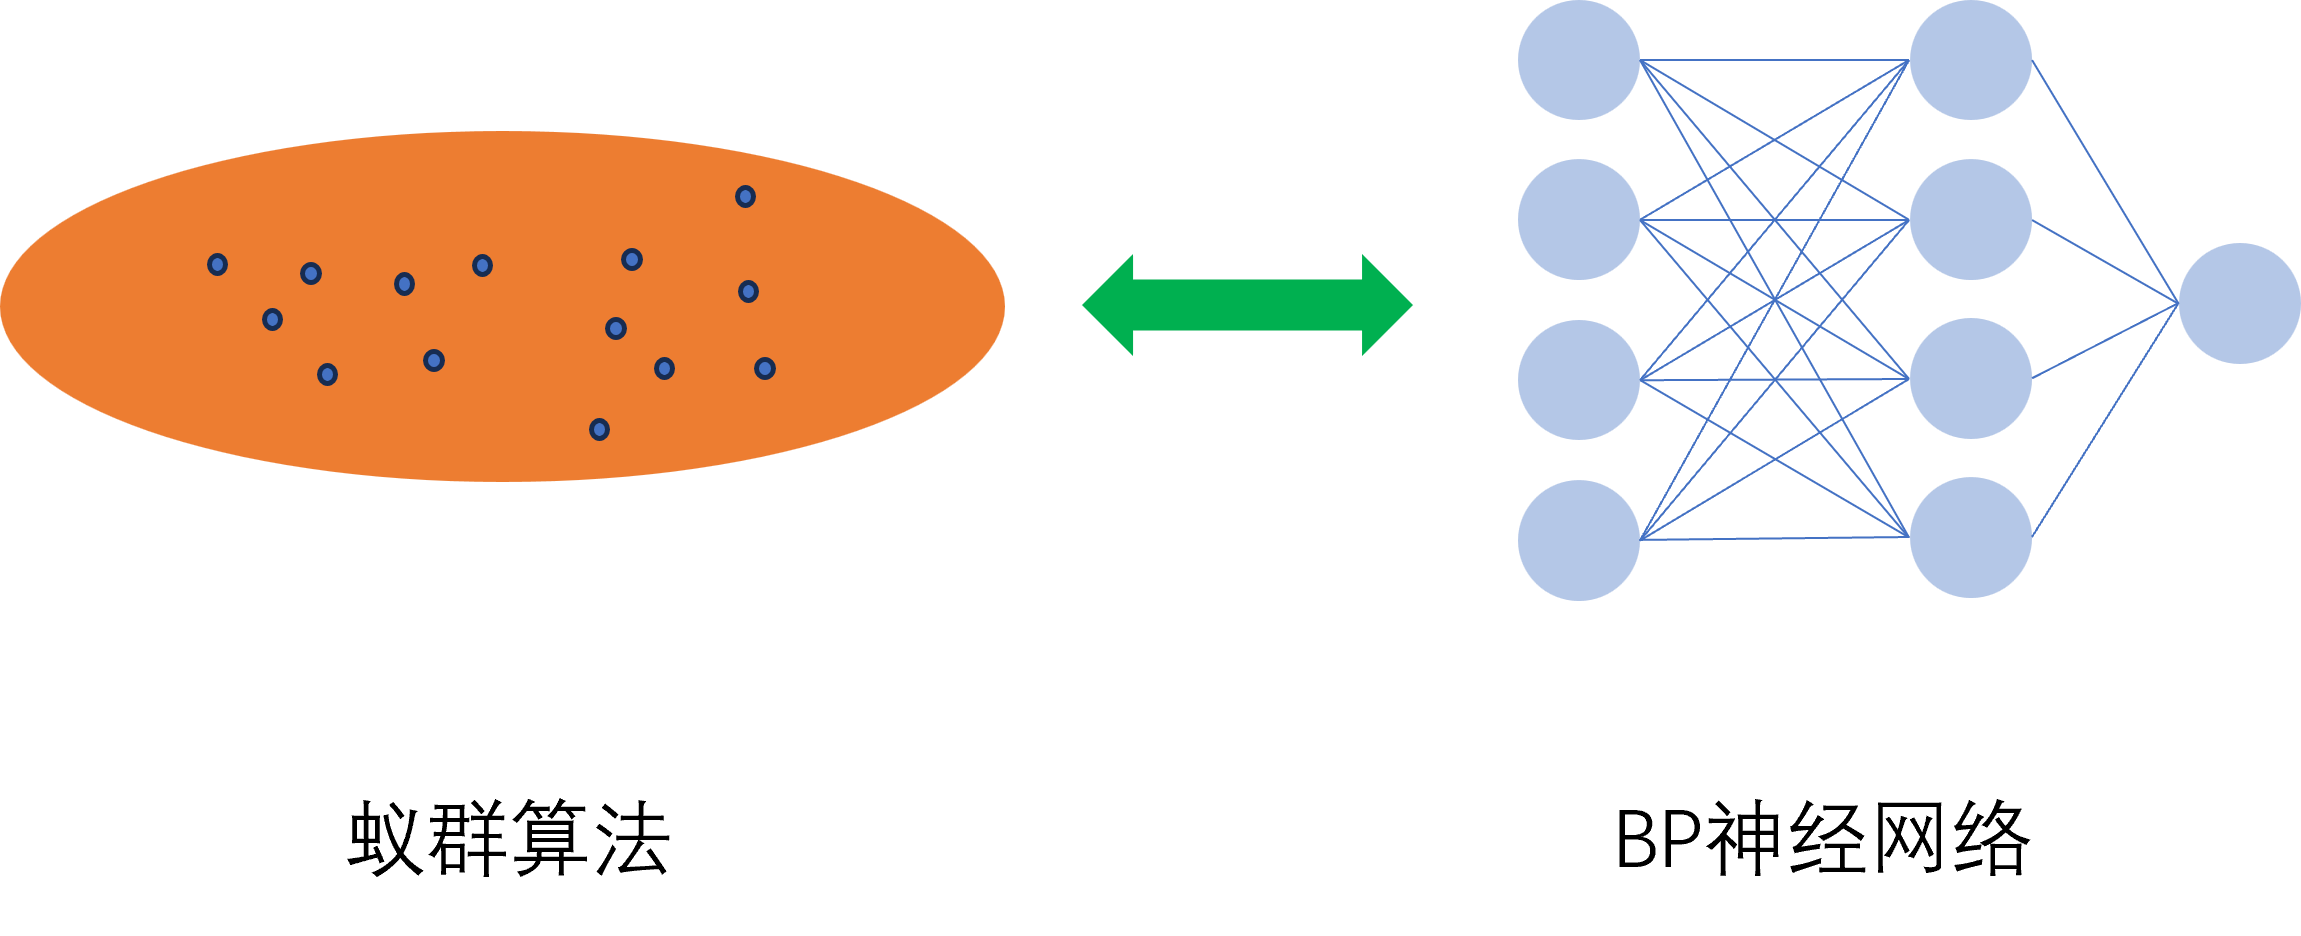
\includegraphics[width=.7\textwidth]{fig_me/蚁群神经网络.png}
  \caption{IACO-BP算法}
  \label{IACO算法}
\end{figure}

\textbf{蚁群部分:}为了加快模型的收敛,本文使用一种改进的蚁群算法优化BP神经网络的运行,具体设置如下:
\begin{itemize}
    \item 随机生成50只蚂蚁,每只蚂蚁代表一个BP神经网络的权重参数组合;
    \item 初始化全局信息素和局部信息素,将它们初始化为0.05;
    \item 每只蚂蚁根据当前权重参数组合计算神经网络的输出,并根据输出结果计算误差值;
    \item 计算每条路径上的选择概率,并根据概率大小选择概率较大的部分蚂蚁的权重参数;
    \item 当所有蚂蚁完成一次搜索后,根据误差函数值更新全局和局部信息素,性能好的蚂蚁释放信息素量更大。
    \item 根据信息素浓度更新BP神经网络的权重参数。
    \item 如果达到了预定的迭代次数或者达到了期望的神经网络性能指标,算法停止。
    
\end{itemize}

\textbf{BP神经网络部分:}
由前文分析得知,原始数据分布不均衡,本文提取原始数据中前100个患者的个人史、疾病史、发病相关指标以及及首次影像结果,利用SMOTE采样防止不均衡数据导致神经网络模型学习过程中出现不可修正的偏差。将SMOTE采样后的矩阵数据与将前100名的mRS数据拼接,并分割训练集和测试集,本文为了防止出现训练集标签不全问题,将随机选取每个mRS等级的20\%作为测试集,传入模型训练,并使用上述蚁群算法进行参数优化。

在前100名患者上,模型预测结果如图~\ref{前100名患者mRS预测结果(只含有首次影像结果)}所示。

\begin{figure}[h] % 使用figure环境,可以让LaTeX自动处理图像的位置
  \centering % 居中放置
  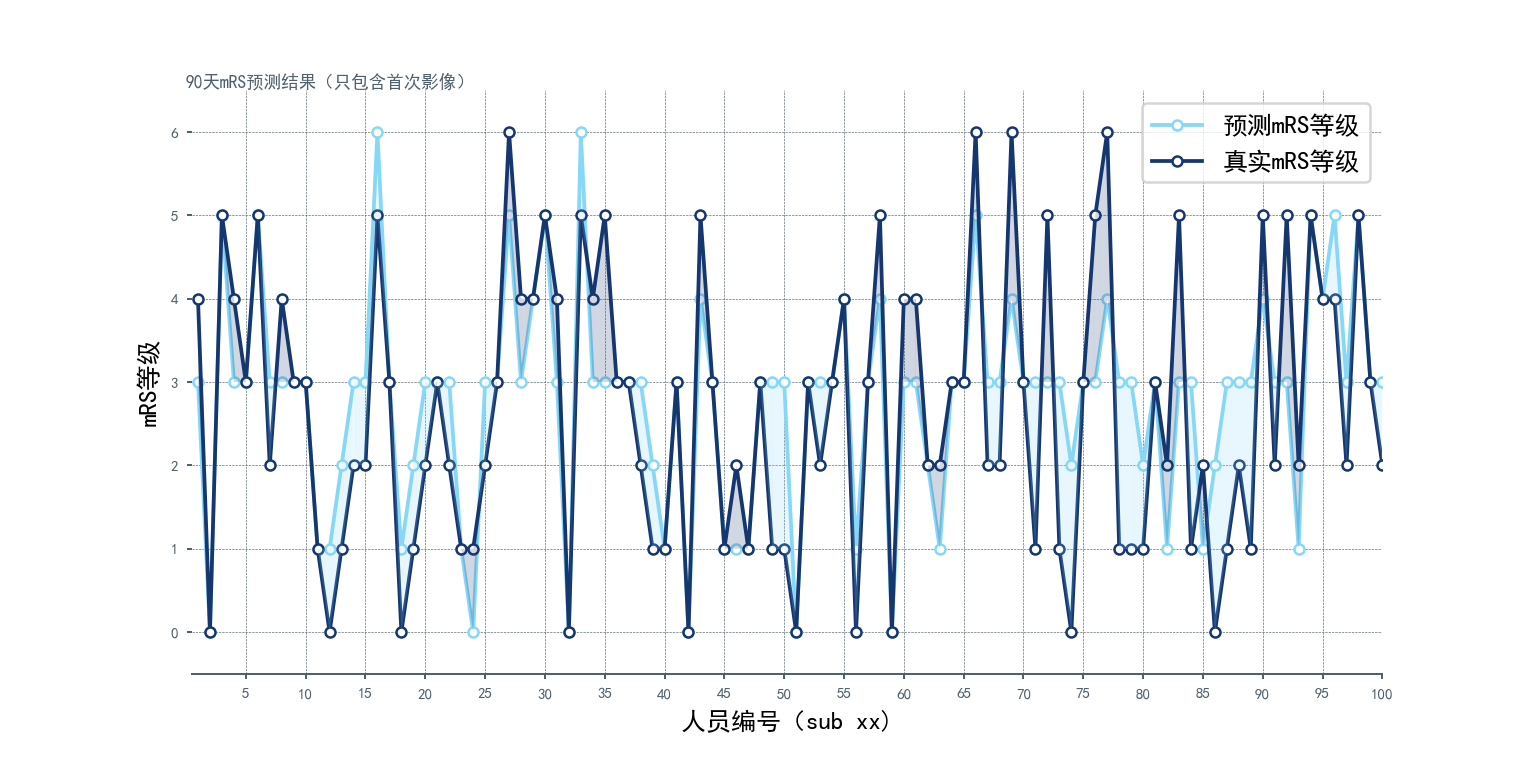
\includegraphics[width=\textwidth]{fig_me/90天mRS预测结果只包含首次影像.png}
  \caption{前100名患者mRS预测结果(只含有首次影像结果)}
  \label{前100名患者mRS预测结果(只含有首次影像结果)}
\end{figure}

对后60名患者mRS预测结果如表~\ref{后60名患者mRS预测结果(只含有首次影像结果)}所示。

\begin{table}[ht]
\caption{后60名患者mRS预测结果(只含有首次影像结果)}
\label{后60名患者mRS预测结果(只含有首次影像结果)}
\centering
\begin{tabular}{cccccccccc}
    \hline
        ID & mRS & ID & mRS & ID & mRS & ID & mRS & ID & mRS \\ \hline
        sub101 & 2 & sub113 & 3 & sub125 & 3 & sub137 & 3 & sub149 & 3 \\ 
        sub102 & 3 & sub114 & 3 & sub126 & 1 & sub138 & 3 & sub150 & 3 \\ 
        sub103 & 5 & sub115 & 6 & sub127 & 3 & sub139 & 3 & sub151 & 3 \\ 
        sub104 & 3 & sub116 & 3 & sub128 & 3 & sub140 & 3 & sub152 & 3 \\ 
        sub105 & 3 & sub117 & 3 & sub129 & 1 & sub141 & 3 & sub153 & 3 \\ 
        sub106 & 2 & sub118 & 3 & sub130 & 3 & sub142 & 3 & sub154 & 3 \\ 
        sub107 & 3 & sub119 & 2 & sub131 & 3 & sub143 & 5 & sub155 & 5 \\ 
        sub108 & 3 & sub120 & 3 & sub132 & 4 & sub144 & 3 & sub156 & 3 \\ 
        sub109 & 3 & sub121 & 4 & sub133 & 3 & sub145 & 2 & sub157 & 3 \\ 
        sub110 & 3 & sub122 & 3 & sub134 & 3 & sub146 & 6 & sub158 & 2 \\ 
        sub111 & 3 & sub123 & 3 & sub135 & 3 & sub147 & 3 & sub159 & 3 \\ 
        sub112 & 3 & sub124 & 3 & sub136 & 3 & sub148 & 3 & sub160 & 3 \\ \hline
    \end{tabular}
\end{table}

\subsubsection{结果分析}

由前100名患者mRS预测结果图(即图~\ref{前100名患者mRS预测结果(只含有首次影像结果)})可知,本文的预测模型虽然准确率不高,但是很多预测错误的患者,mRS等级也与真实值相仿,基本落在上下一个等级范围内,从该角度看,本文的预测模型较为精准。在后60名患者的预测结果上,90天mRS大多数为3,属于是较为正常的预测,落于较高等级的患者需要重点关注。

\subsection{模型3b的建立与求解}
\subsubsection{相关模型}

\textbf{长短期记忆网络模型(LSTM)}\cite{LSTM}是一种用于处理长期依赖关系的循环神经网络(RNN)模型。相比传统的RNN模型,LSTM在处理长序列数据时具有更好的记忆性能。LSTM通过引入门控机制(gate mechanism)来控制信息的流动,从而解决了传统RNN模型在长序列上容易发生梯度消失或梯度爆炸的问题。LSTM主要包含以下几个关键部分:


遗忘门:
\begin{equation}
f(t) = \sigma(W_f \cdot [h(t-1), x(t)] + b_f)
\end{equation}

输入门:
\begin{equation}
i(t) = \sigma(W_i \cdot [h(t-1), x(t)] + b_i)
\end{equation}
\begin{equation}
\hat{C}(t) = \tanh(W_{\hat{C}} \cdot [h(t-1), x(t)] + b_{\hat{C}})
\end{equation}

输出门:
\begin{equation}
o(t) = \sigma(W_o \cdot [h(t-1), x(t), dt] + b_o)
\end{equation}

当前时刻记忆:
\begin{equation}
c(t) = f(t) \cdot c(t-1) + i(t) \cdot \hat{C}(t)
\end{equation}

当前时刻隐藏状态:
\begin{equation}
h(t) = o(t) \cdot \tanh(c(t))
\end{equation}

其中,$W$表示权重矩阵,$b$表示偏置向量,$\sigma$表示sigmoid函数,$*$表示按位乘法,$[]$表示连接操作。


\subsubsection{模型建立}
本节提取了前100个患者所有已知临床、治疗指标数据以及所有影像结果,首先观察到该部分数据中,所有已知临床、治疗指标数据均为不具有时间属性的数据,而所有影像结果均具有时间属性,考虑到数据所带有的时间属性可能对模型预测结果的影响,本文在节~\ref{IACO-BP}的模型基础上加入了LSTM模型,首先切割数据,一份为所有已知临床、治疗指标数据以及首次影像结果数据,另一份为所有影像数据,包括所有影像检查时间数据。第一份数据使用节~\ref{IACO-BP}中建立的算法进行预测模型的建立。而对于第二份数据,本文使用LSTM算法建立纵向数据的预测模型,并使用蚁群算法进行有优化。最后,使用投票算法将基于LSTM的mRS预测模型和基于BP的mRS预测模型进行融合。

算法框架如下:
\begin{figure}[h] % 使用figure环境,可以让LaTeX自动处理图像的位置
  \centering % 居中放置
  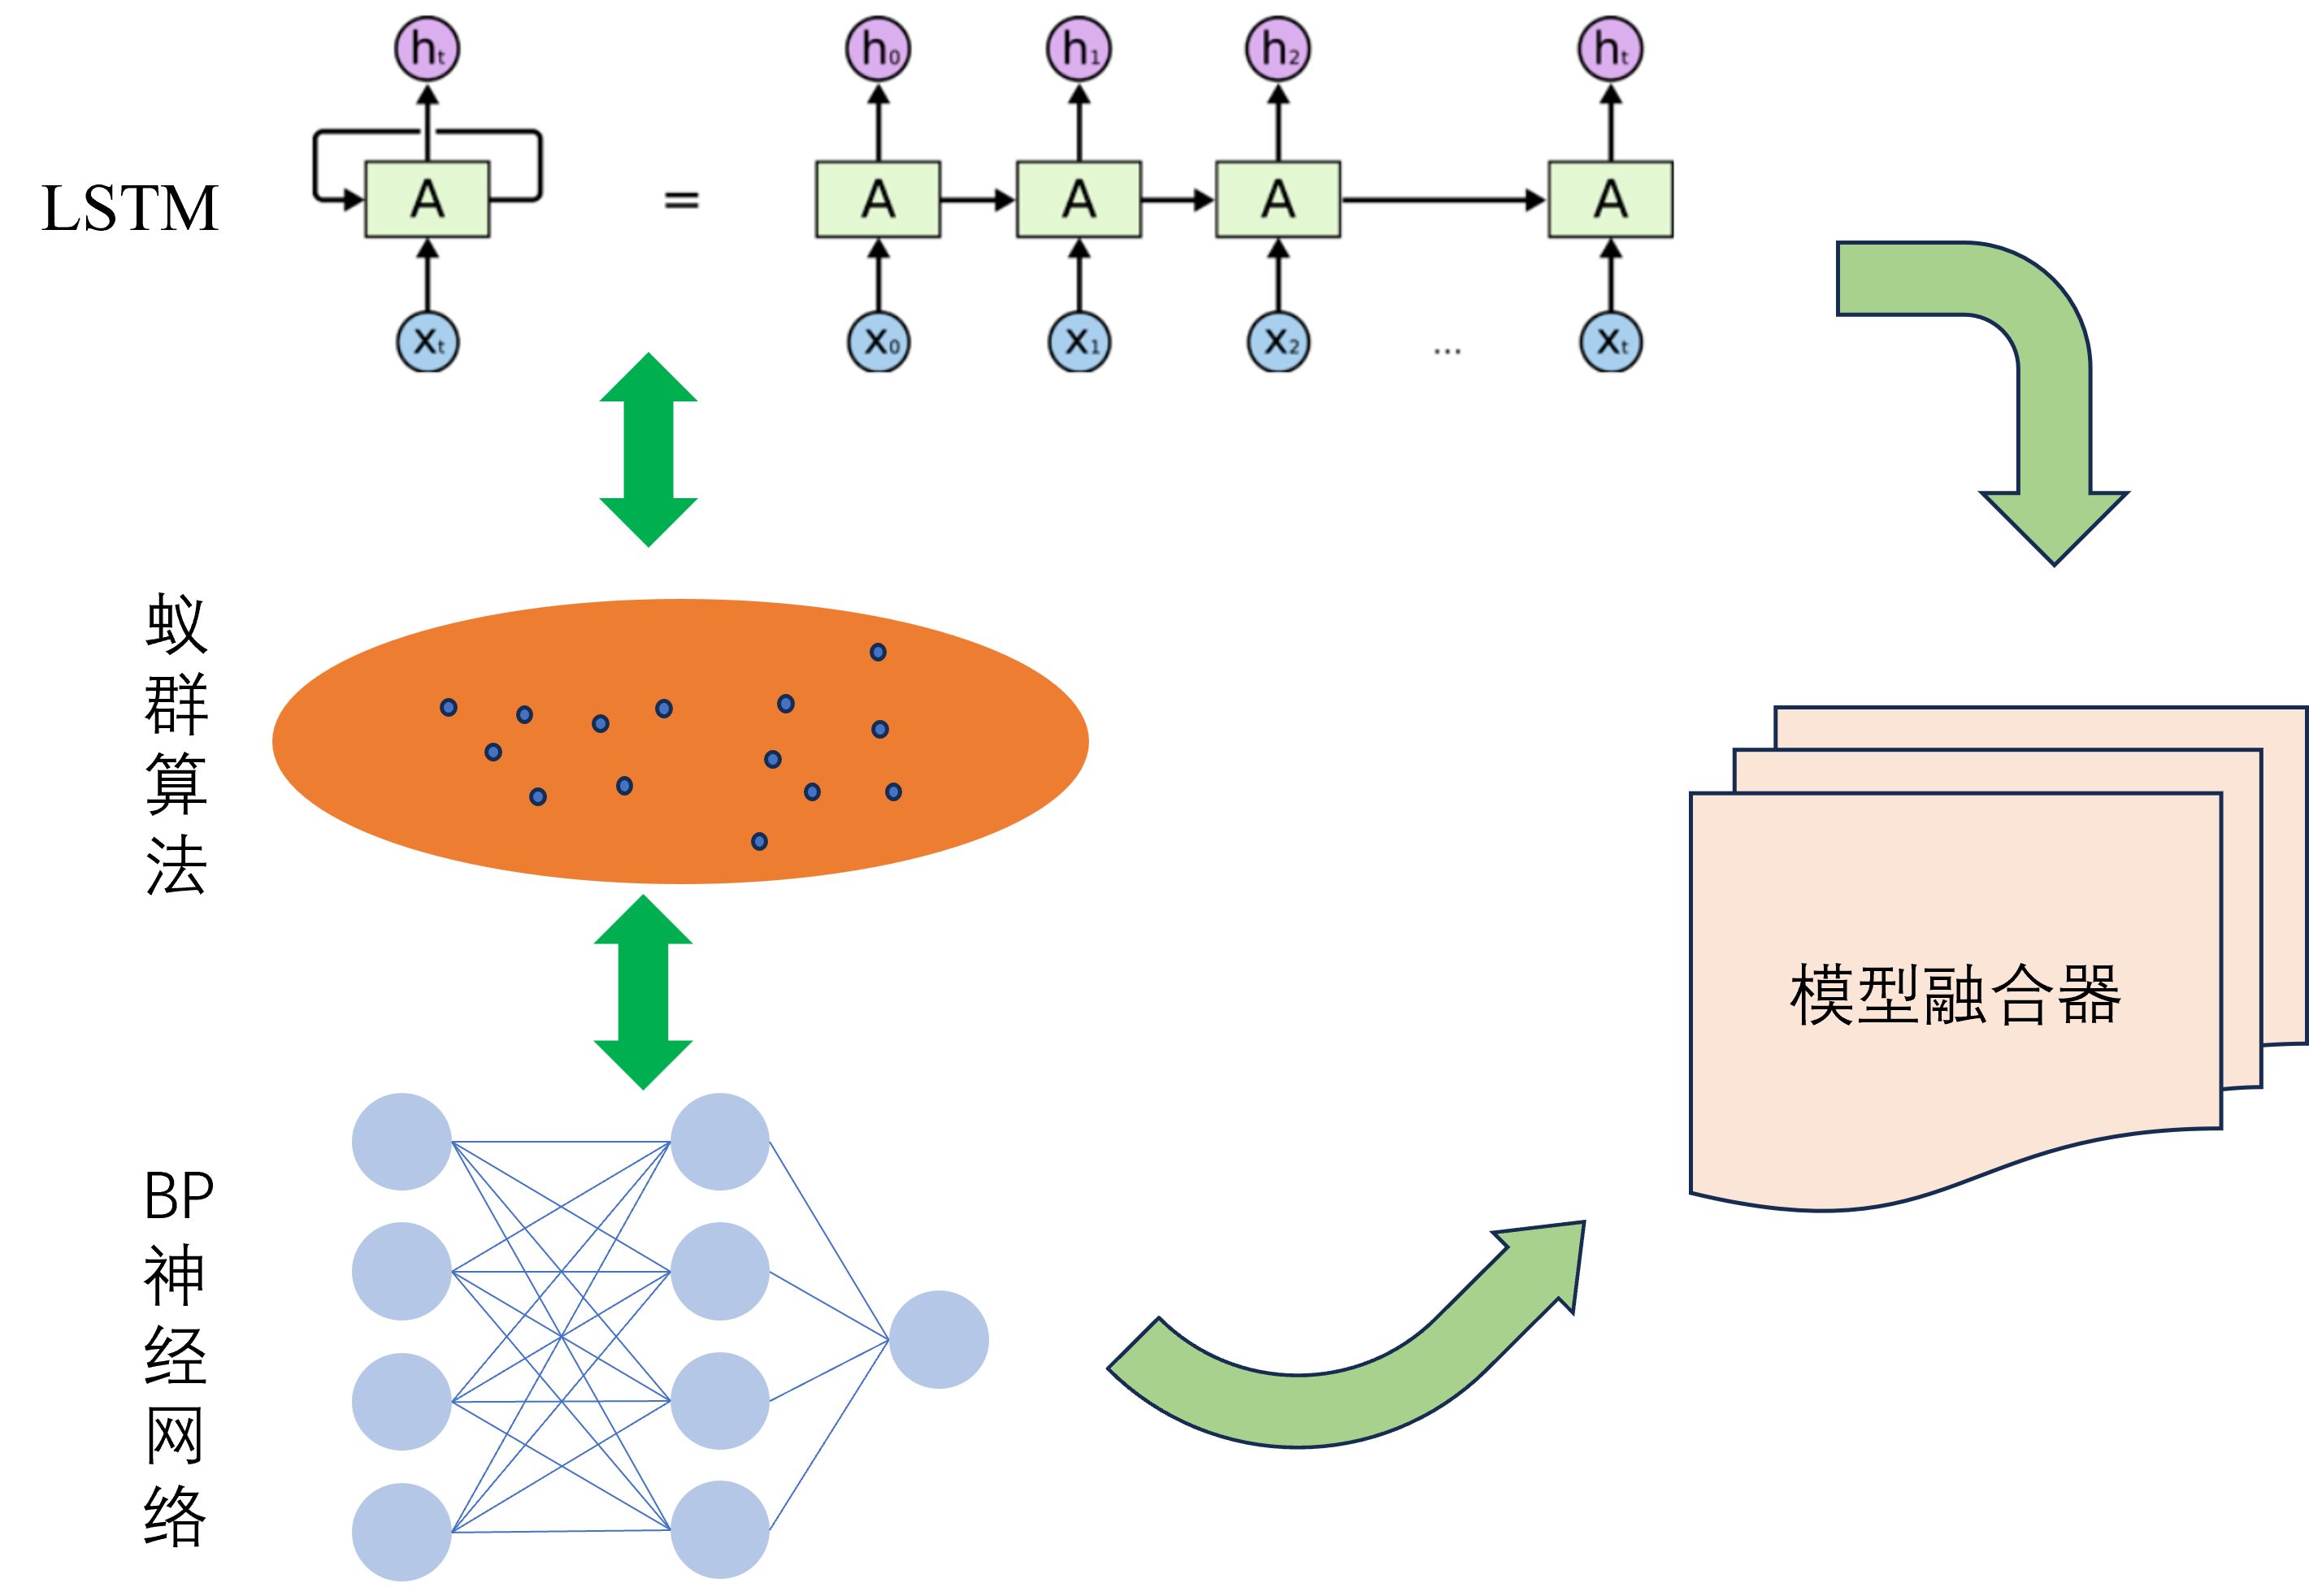
\includegraphics[width=.7\textwidth]{fig_me/融合模型.png}
  \caption{LSTM-IACO-BP融合算法}
  \label{LSTM-IACO-BP融合算法}
\end{figure}

观察到影像检查结果数据的时间间隔不是固定的,本文在传统的LSTM算法上引入了模糊时间项$dt$,而LSTM的几个重要部分将变为如下:

遗忘门:
\begin{equation}
f(t) = \sigma(W_f \cdot [h(t-1), x(t), dt] + b_f)
\end{equation}

输入门:
\begin{equation}
i(t) = \sigma(W_i \cdot [h(t-1), x(t), dt] + b_i)
\end{equation}
\begin{equation}
\hat{C}(t) = \tanh(W_{\hat{C}} \cdot [h(t-1), x(t), dt] + b_{\hat{C}})
\end{equation}

输出门:
\begin{equation}
o(t) = \sigma(W_o \cdot [h(t-1), x(t), dt] + b_o)
\end{equation}

当前时刻记忆:
\begin{equation}
c(t) = f(t) \cdot c(t-1) + i(t) \cdot \hat{C}(t)
\end{equation}

当前时刻隐藏状态:
\begin{equation}
h(t) = o(t) \cdot \tanh(c(t))
\end{equation}

其中,$dt$表示模糊时间间隔。在这种情况下,模型可以通过学习到的权重来适应不同的时间间隔,从而更好地处理具有模糊时间概念的数据。



\subsubsection{模型求解}


由前文分析得知,原始数据分布不均衡,本文提取原始数据中前100个患者的个人史、疾病史、发病相关指标以及及首次影像结果,利用SMOTE采样防止不均衡数据导入BP神经网络模型学习过程中出现不可修正的偏差。将SMOTE采样后的矩阵数据与将前100名的mRS数据拼接,并分割训练集和测试集,本文为了防止出现训练集标签不全问题,将随机选取每个mRS等级的20\%作为测试集,传入模型训练,并使用节~\ref{IACO算法}介绍的蚁群算法进行参数优化。紧接着提取原始数据中前100个患者的所有影像结果,利用SMOTE采样防止不均衡数据导入LSTM模型学习过程中出现不可修正的偏差。将SMOTE采样后的矩阵数据与将前100名的mRS数据拼接,并分割训练集和测试集,本文为了防止出现训练集标签不全问题,将随机选取每个mRS等级的20\%作为测试集,传入模型训练,并使用节~\ref{IACO算法}介绍的蚁群算法进行参数优化。

在前100名患者上,模型预测结果如图~\ref{前100名患者mRS预测结果(包含首次+随访影像)}所示。对后30名患者mRS预测结果如表~\ref{后30名患者mRS预测结果(包含首次+随访影像)}所示。

\begin{figure}[h] % 使用figure环境,可以让LaTeX自动处理图像的位置
  \centering % 居中放置
  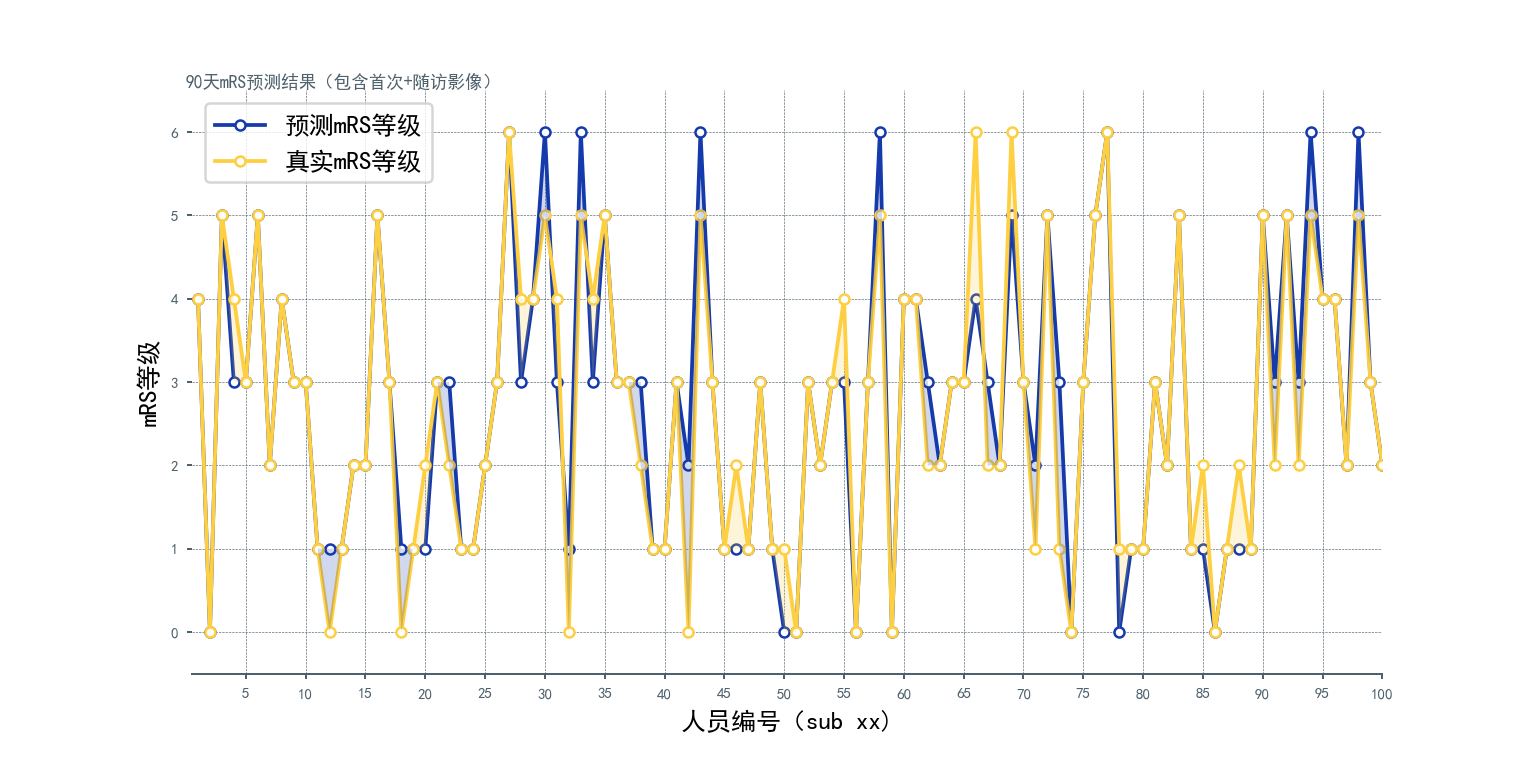
\includegraphics[width=\textwidth]{fig_me/90天mRS预测结果(包含首次+随访影像).png}
  \caption{前100名患者mRS预测结果(包含首次+随访影像)}
  \label{前100名患者mRS预测结果(包含首次+随访影像)}
\end{figure}

\begin{table}[ht]
\caption{后30名患者mRS预测结果(包含首次+随访影像)}
\label{后30名患者mRS预测结果(包含首次+随访影像)}
\centering
\begin{tabular}{cccc}
     \hline
        ID & mRS & ~ & mRS \\ \hline
        sub131 & 5 & sub146 & 4 \\ 
        sub132 & 5 & sub147 & 5 \\ 
        sub133 & 3 & sub148 & 3 \\ 
        sub134 & 3 & sub149 & 5 \\ 
        sub135 & 2 & sub150 & 5 \\ 
        sub136 & 3 & sub151 & 3 \\ 
        sub137 & 3 & sub152 & 5 \\ 
        sub138 & 3 & sub153 & 1 \\ 
        sub139 & 2 & sub154 & 3 \\ 
        sub140 & 3 & sub155 & 3 \\ 
        sub141 & 3 & sub156 & 3 \\ 
        sub142 & 3 & sub157 & 3 \\ 
        sub143 & 3 & sub158 & 3 \\ 
        sub144 & 5 & sub159 & 5 \\ 
        sub145 & 3 & sub160 & 5 \\ \hline
    \end{tabular}
\end{table}

\subsubsection{结果分析}

由前100名患者mRS预测结果图(即图~\ref{前100名患者mRS预测结果(包含首次+随访影像)})可知,模型预测精度较上一问结果有所提高,但仍然有不够精确。在后30名患者的预测结果上,90天mRS与上一问结果相差较大,由考虑到在前100名患者的mRS预测结果比上一问好,所以本文更倾向于相信本节的算法。

\subsection{模型3c的建立与求解}
\subsubsection{相关模型}

\textbf{Shapiro-Wilk 分布检验模型}:

Shapiro-Wilk 分布检验模型\cite{Shapiro-Wilk}的零检验是:样本$X_1,X_2,...,X_n$来自于一个同一总体,且总体服从正态分布。其中,检验统计量是:

\begin{equation}
W=\frac{\left(\sum_{i=1}^na_ix_{(i)}\right)^2}{\sum_{i-1}^n(x_i-\bar{x})^2}
\end{equation}

\noindent 其中:$x_{(i)}$即样本中的第i个最小数。$\bar{x}$是样本的平均值。常量$a_i$通过下述公式计算:

\begin{equation}
(a_1,...,a_n)=\frac{m^{\mathsf{T}}V^{-1}}{(m^{\mathsf{T}}V^{-1}V^{-1}m)^{1/2}}
\end{equation}


\textbf{Kruskal-Wallis H检验模型}:

Kruskal-Wallis H检验模型\cite{Kruskal-Wallis-H}用于检验多个总体的分布是否存在显著差异。
原理是:将多组样本数据混合并排序,求出各变量值的秩。判断各组秩的均值是否存在显著差异。具体流程如下:


构建原假设:

\begin{equation}
H_0{:}\mu_1=\mu_2=...\mu_k
\end{equation}

构建备择假设$H_1$:

\begin{equation}
H_1{:}\mu_{i}\neq\mu_{j}
\end{equation}

构建检验统计量:

\begin{equation}
H=\frac{12}{N(N+1)}\sum_{i=1}^kn_i(\overline{R}_i-\overline{R})^2=\frac{12}{N(N+1)}\sum_{i=1}^kn_i\overline{R}_i^2-3(N+1)\sim\chi^2(k-1)
\end{equation}



\subsubsection{模型建立}



针对样本数据,以“数据的分布具有正态性”为原假设($H_0$),进行Kolmogorov-Smirnov分布检验。


其中,假设总体的分布函数为 F(x),是一个连续函数,而样本来自这个总体。那么,样本的累积分布函数可以表示为 S(x):

\begin{equation}
F_n(x)=\frac{1}{n}\sum_{i=1}^nI_{[-\infty,x]}(X_i)
\end{equation}

\noindent 其中,$I_{[-\text{inf,}x]}$为指示函数,其取值为:

\begin{equation}
\left.\mathrm{I_{[-inf,x]}(X_i)}=\left\{\begin{matrix}1,X_i\leq x\\0,X_i>x\end{matrix}\right.\right.
\end{equation}

进一步地,Kolmogorov-Smirnov统计量可被表述为:

\begin{equation}
D_n=sup_x|F_n(x)-F(x)|
\end{equation}

\noindent 若$X_i$服从$F(x)$,当n趋于无穷,$D_n$趋近于0。显著性取0.05。若检验值小于0.05,则该指标的分布不具有正态性。

\subsubsection{模型求解}

1)若有序变量服从正太分布,变量间的总体皮尔逊相关系数定义如公式集:

\begin{equation}
\rho_{X,Y}=\frac{\operatorname{cov}\left(X,Y\right)}{\sigma_X\sigma_Y}=\frac{E[(X-\mu_X)(Y-\mu_Y)]}{\sigma_X\sigma_Y}
\end{equation}

$\rho_{X,Y}$为两个变量之间的协方差,$\sigma_X\sigma_Y$为两个变量的标准差的乘积。

样本皮尔逊相关系数定义如公式集:

\begin{equation}
[\sum_{i=1}^n(X_i-\overline{X})(Y_i-\overline{Y})]/[{\sqrt{\sum_{i=1}^n(X_i-\overline{X})^2}\sqrt{\sum_{i=1}^n(Y_i-\overline{Y})^2}}]
\end{equation}



\noindent 其中,$\frac{X_{i}-\overline{X}}{\sigma_{X}}$,$\overline{X}$及$sigma_X$分别是$X_i$样本的标准分数、样本平均值和样本标准差。

2)若有序变量不服从正太分布,首先计算斯皮尔曼相关系数:

\begin{equation}
r_s=1-\frac{6\sum_{i=1}^nd_i^2}{n(n^2-1)}
\end{equation}

\noindent 其中n是样本的数量,d代表数据x和y之间的等级差。

3)对于无序变量,需要进行方差齐性检验,Kruskal-Wallis H检验。检验过程如下:

以“满足方差齐性”作为$H_0$假设,即:

\begin{equation}
m_1=m_2=\cdots=m_r=m
\end{equation}

其中,m为实验重复次数。同方差条件下,记H分布为H(r,f),获取H(r,f)分位数。若$H_0$成立,有:

\begin{equation}
\sigma_1^2=\sigma_2^2=\cdots=\sigma_r^2
\end{equation}

$H_0$的拒绝域为:

\begin{equation}
W_1=\{H>H_{1-\alpha}(r,f)\}
\end{equation}

\noindent 其中$H>H_{1-\alpha}(r,f)$为H分布的分位数.

4)无序变量中的数据既不服从正态分布,也不满足方差齐性:
使用Kruskal-Wallis H检验判断相关性。


\subsubsection{结果分析}



1)相关性分析:90天mRS与无序变量

分析有序变量与90天mRS之间的联系之前,本文针对无序变量单独进行相关性分析:

通常情况下,使用Kolmogorov-Smirnov检验来进行显著性测试。简而言之,如果检验的P值小于0.05,将拒绝零假设,表明该指标的数据不符合正态分布。下文以性别与其他变量的关系为例进行详细分析,本文首先进行了正态性检验,其结果如下表~\ref{正态性检验}。


\begin{table}[!ht]
    \centering
    \caption{正态性检验}
    \label{正态性检验}
    \begin{tabular}{cc}
        \toprule
        指标 & 显著性 \\
        \midrule
        90天mRS & 3.1867E-18 \\
        \bottomrule
    \end{tabular}
\end{table}



基于p值,本文拒绝零假设$H_0$,即90天mRS不服从正态分布。其中,方差齐性检验P值如表~\ref{方差齐性检验}。

\begin{table}[!ht]
    \centering
    \caption{方差齐性检验}
    \label{方差齐性检验}
    \begin{tabular}{lcc}
    \hline
        &莱文统计 & 显著性 \\ \hline
        90天mRS & 167.13789 & 2.78E-145 \\ \hline
    \end{tabular}
\end{table}

基于莱文统计显著性值,本文得出合理推断:数据不满足方差齐性。综上,无序变量中的数据不服从正态分布,也不满足方差齐性,因此本文使用Kruskal-Wallis H检验判断相关性。

Kruskal-Wallis H检验分析结果如表~\ref{KW检验分析}。

\begin{table}[!ht]
    \centering
    \caption{KW检验分析}
    \label{KW检验分析}
    \begin{tabular}{lc}
    \toprule
        $$$$ & 值 \\
    \midrule
        H & 2416.23624 \\
        p & 0.49245 \\
    \bottomrule
    \end{tabular}
\end{table}

基于显著性值,本文得出结论:90天mRS与性别无关。

2)相关性分析:90天mRS与有序变量


鉴于该样本量数据较小,本文基于Shapiro–Wilk检验讨论数据的正态性。
正态性检验结果如表~\ref{指标显著性表}(见附录)所示。
基于斯皮尔曼相关系数对相关性进行分析,绘制相关性热力图,将结果以直观图表形式呈现,分析结果如图~\ref{相关性热力图}所示。

\begin{figure}[h] % 使用figure环境,可以让LaTeX自动处理图像的位置
  \centering % 居中放置
  \includegraphics[width=.7\textwidth]{figures/热力图.png}
  \caption{相关性热力图}
  \label{相关性热力图}
\end{figure}



\newpage
%参考文献   手工录入
%\begin{thebibliography}{9}%宽度9
% \bibitem{bib:one} ....
% \bibitem{bib:two} ....
%\end{thebibliography}

%采用bibtex方案
% \cite{mittelbach_latex_2004,wright_latex3_2009,beeton_unicode_2008,vieth_experiences_2009}

\bibliographystyle{gmcm}
\bibliography{example}


\newpage
%附录
\appendix
% \setcounter{page}{1} %如果需要可以自行重置页码。
\section{附表}

\begin{table}[!ht]
    \centering
    % \renewcommand{\arraystretch}{0.2} % 设置行高
    
    \begin{spacing}{0.6}
    \caption{组合治疗分组对照表}
    \label{组合治疗分组对照表}
    \begin{tabular}{cccccccc}
    \toprule[1.5pt]   % 上边线(或表示为)
        \small{组别} & \small{脑室引流} & \small{止血治疗} & \small{降颅压治疗} & \small{降压治疗} & \small{镇静、镇痛治疗} & \small{止吐护胃} & {营养神经} \\ 
        \midrule[1pt]
        1 & - & - & - & - & - & √ & √ \\ 
        2 & - & - & √ & √ & - & - & - \\ 
        3 & - & √ & - & - & - & √ & - \\ 
        4 & - & √ & √ & √ & - & - & - \\ 
        5 & - & √ & - & √ & - & - & √ \\ 
        6 & - & - & √ & - & √ & √ & - \\ 
        7 & - & - & √ & √ & - & √ & - \\ 
        8 & - & - & - & - & √ & √ & √ \\ 
        9 & - & - & - & √ & - & √ & √ \\ 
        10 & - & √ & - & - & - & √ & √ \\ 
        11 & - & - & √ & - & - & √ & √ \\ 
        12 & - & √ & √ & - & - & √ & - \\ 
        13 & - & - & √ & √ & - & - & √ \\ 
        14 & - & √ & √ & - & - & √ & √ \\ 
        15 & √ & - & - & √ & - & √ & √ \\ 
        16 & - & - & √ & √ & - & √ & √ \\ 
        17 & - & - & - & √ & √ & √ & √ \\ 
        18 & - & √ & √ & √ & - & - & √ \\ 
        19 & - & √ & - & √ & - & √ & √ \\ 
        20 & - & √ & √ & √ & - & √ & √ \\ 
        21 & - & √ & - & √ & √ & √ & √ \\ 
        22 & - & √ & √ & √ & √ & √ & - \\ 
        23 & - & - & √ & √ & √ & √ & √ \\ 
        24 & √ & - & - & √ & √ & √ & √ \\ 
        25 & √ & - & √ & √ & - & √ & √ \\ 
        26 & - & √ & √ & √ & √ & √ & √ \\ 
        27 & √ & - & √ & √ & √ & √ & √ \\ 
        28 & √ & √ & √ & √ & √ & √ & √ \\ 
        \bottomrule[1.5pt] 
    \end{tabular}
    \end{spacing}
    
\end{table}

\begin{table}[htbp]
  \scriptsize
  \centering
  \caption{是否扩张及扩张概率}
  \label{是否扩张及扩张概率_全表}
  \begin{tabular}{cccccc}
    \toprule
    ID & 是否发生血肿扩张 & 血肿扩张预测概率 & ID & 是否发生血肿扩张 & 血肿扩张预测概率 \\
    \midrule
    sub001 & 0 & 0.0199 & sub051 & 0 & 0.013 \\
    sub002 & 0 & 0.009 & sub052 & 0 & 0.0366 \\
    sub003 & 1 & 0.9487 & sub053 & 0 & 0.0107 \\
    sub004 & 0 & 0.0107 & sub054 & 1 & 0.993 \\
    sub005 & 1 & 0.987 & sub055 & 0 & 0.0322 \\
    sub006 & 0 & 0.0152 & sub056 & 0 & 0.0098 \\
    sub007 & 0 & 0.014 & sub057 & 1 & 0.9711 \\
    sub008 & 1 & 0.9743 & sub058 & 1 & 0.973 \\
    sub009 & 1 & 0.9968 & sub059 & 0 & 0.0069 \\
    sub010 & 0 & 0.0395 & sub060 & 1 & 0.9784 \\
    sub011 & 0 & 0.0256 & sub061 & 1 & 0.9844 \\
    sub012 & 0 & 0.0153 & sub062 & 0 & 0.0197 \\
    sub013 & 1 & 0.9596 & sub063 & 1 & 0.9447 \\
    sub014 & 0 & 0.0226 & sub064 & 0 & 0.0111 \\
    sub015 & 1 & 0.9834 & sub065 & 1 & 0.9377 \\
    sub016 & 0 & 0.0174 & sub066 & 0 & 0.0221 \\
    sub017 & 1 & 0.9928 & sub067 & 0 & 0.0062 \\
    sub018 & 1 & 0.9868 & sub068 & 0 & 0.0266 \\
    sub019 & 0 & 0.0157 & sub069 & 0 & 0.0256 \\
    sub020 & 0 & 0.0386 & sub070 & 1 & 0.9767 \\
    sub021 & 0 & 0.0092 & sub071 & 1 & 0.9596 \\
    sub022 & 0 & 0.0364 & sub072 & 0 & 0.0175 \\
    sub023 & 0 & 0.0336 & sub073 & 0 & 0.0033 \\
    sub024 & 0 & 0.0106 & sub074 & 1 & 0.9593 \\
    sub025 & 1 & 0.9869 & sub075 & 0 & 0.0367 \\
    sub026 & 0 & 0.0148 & sub076 & 1 & 0.9541 \\
    sub027 & 1 & 0.9548 & sub077 & 0 & 0.0143 \\
    sub028 & 0 & 0.001 & sub078 & 0 & 0.0488 \\
    sub029 & 0 & 0.0095 & sub079 & 1 & 0.9502 \\
    sub030 & 0 & 0.033 & sub080 & 1 & 0.9872 \\
    sub031 & 0 & 0.0065 & sub081 & 1 & 0.9824 \\
    sub032 & 1 & 0.987 & sub082 & 0 & 0.0036 \\
    sub033 & 1 & 0.9574 & sub083 & 0 & 0.0049 \\
    sub034 & 0 & 0.0033 & sub084 & 1 & 0.9939 \\
    sub035 & 0 & 0.0077 & sub085 & 0 & 0.0118 \\
    sub036 & 1 & 0.9753 & sub086 & 0 & 0.0228 \\
    sub037 & 1 & 0.9922 & sub087 & 1 & 0.9905 \\
    sub038 & 1 & 0.9653 & sub088 & 0 & 0.0155 \\
    sub039 & 1 & 0.9986 & sub089 & 0 & 0.0308 \\
    sub040 & 0 & 0.074 & sub090 & 0 & 0.0301 \\
    sub041 & 0 & 0.0249 & sub091 & 0 & 0.039 \\
    sub042 & 0 & 0.0047 & sub092 & 1 & 0.976 \\
    sub043 & 1 & 0.9901 & sub093 & 0 & 0.0163 \\
    sub044 & 0 & 0.0112 & sub094 & 0 & 0.0193 \\
    sub045 & 0 & 0.02 & sub095 & 0 & 0.0089 \\
    sub046 & 0 & 0.0022 & sub096 & 0 & 0.0299 \\
    sub047 & 1 & 0.9632 & sub097 & 0 & 0.0217 \\
    sub048 & 1 & 0.9799 & sub098 & 0 & 0.0167 \\
    sub049 & 0 & 0.004 & sub099 & 1 & 0.9745 \\
    sub050 & 0 & 0.0211 & sub100 & 0 & 0.0052 \\
    \bottomrule
  \end{tabular}
\end{table}


\begin{table}[ht]
\caption{组合治疗方法的回归系数及显著性}
\label{组合治疗方法的回归系数及显著性}
\centering
\begin{tabular}{lcccccc}
\toprule
& Coef & Std Err & t & P>|t| & [0.025 & 0.975] \\
\midrule
const & -0.2331 & 0.537 & -0.434 & 0.666 & -1.302 & 0.836 \\
治疗组合1 & -0.3584 & 0.508 & -0.705 & 0.483 & -1.369 & 0.652 \\
治疗组合2 & 0.0618 & 0.565 & 0.109 & 0.913 & -1.062 & 1.186 \\
治疗组合3 & -0.6384 & 0.648 & -0.985 & 0.328 & -1.928 & 0.651 \\
治疗组合4 & -0.8287 & 0.813 & -1.020 & 0.311 & -2.445 & 0.788 \\
治疗组合5 & 1.2331 & 0.823 & 1.498 & 0.138 & -0.405 & 2.871 \\
治疗组合6 & -0.1285 & 0.537 & -0.239 & 0.812 & -1.197 & 0.940 \\
治疗组合7 & 1.1713 & 0.736 & 1.592 & 0.115 & -0.293 & 2.635 \\
治疗组合8 & -0.0085 & 0.427 & -0.020 & 0.984 & -0.859 & 0.842 \\
治疗组合9 & -0.0615 & 0.424 & -0.145 & 0.885 & -0.905 & 0.782 \\
治疗组合10 & -0.2844 & 0.504 & -0.564 & 0.574 & -1.287 & 0.718 \\
治疗组合11 & 0.1132 & 0.536 & 0.211 & 0.833 & -0.953 & 1.179 \\
治疗组合12 & 0.6538 & 0.705 & 0.927 & 0.357 & -0.750 & 2.057 \\
治疗组合13 & 0.5664 & 0.680 & 0.833 & 0.407 & -0.786 & 1.918 \\
治疗组合14 & -0.2527 & 0.449 & -0.563 & 0.575 & -1.146 & 0.641 \\
治疗组合15 & -0.3471 & 0.852 & -0.407 & 0.685 & -2.043 & 1.348 \\
治疗组合16 & -0.2598 & 0.788 & -0.330 & 0.742 & -1.827 & 1.308 \\
治疗组合17 & 0.6615 & 0.448 & 1.478 & 0.143 & -0.229 & 1.552 \\
治疗组合18 & 0.2005 & 0.940 & 0.213 & 0.832 & -1.669 & 2.070 \\
治疗组合19 & -0.6574 & 0.465 & -1.413 & 0.161 & -1.583 & 0.268 \\
治疗组合20 & -0.6258 & 0.645 & -0.970 & 0.335 & -1.909 & 0.658 \\
治疗组合21 & 0.2255 & 0.654 & 0.345 & 0.731 & -1.075 & 1.526 \\
治疗组合22 & 0.9418 & 0.693 & 1.360 & 0.178 & -0.436 & 2.319 \\
治疗组合23 & -1.4529 & 0.769 & -1.890 & 0.062 & -2.982 & 0.076 \\
治疗组合24 & 1.3471 & 1.166 & 1.155 & 0.251 & -0.972 & 3.666 \\
治疗组合25 & -0.3580 & 0.404 & -0.886 & 0.378 & -1.162 & 0.446 \\
治疗组合26 & 0.0352 & 0.758 & 0.046 & 0.963 & -1.473 & 1.544 \\
治疗组合27 & -0.3580 & 0.404 & -0.886 & 0.378 & -1.162 & 0.446 \\
治疗组合28 & -0.3580 & 0.404 & -0.886 & 0.378 & -1.162 & 0.446 \\
\bottomrule
\end{tabular}
\end{table}




\begin{table}[!ht]
    \centering
    \begin{spacing}{0.7}
    \caption{分组残差表}
    \label{分组残差表}
    \begin{tabular}{ccccccccc}
    \hline
        ID & 残差 & 分组情况 & ID & 残差 & 分组情况 & ID & 残差 & 分组情况 \\ \hline
        sub001 & 249.5368 & 2 & sub034 & 101.1988 & 2 & sub068 & 43.8177 & 2 \\ 
        sub002 & 16.3403 & 4 & sub035 & 90.2611 & 3 & sub069 & 96.8805 & 3 \\ 
        sub003 & 48.1681 & 2 & sub036 & 83.1129 & 2 & sub070 & 15.5481 & 1 \\ 
        sub004 & 49.0047 & 4 & sub037 & 60.9421 & 2 & sub071 & 112.1994 & 1 \\ 
        sub005 & 45.5488 & 4 & sub038 & 68.3904 & 2 & sub072 & 31.5675 & 1 \\ 
        sub006 & 199.9552 & 1 & sub039 & 222.7279 & 2 & sub073 & 66.8155 & 2 \\ 
        sub007 & 52.8367 & 3 & sub040 & 92.7453 & 2 & sub074 & 179.5602 & 2 \\ 
        sub008 & 103.9248 & 0 & sub041 & 95.7108 & 2 & sub075 & 33.1681 & 1 \\ 
        sub009 & 27.8458 & 4 & sub042 & 15.9246 & 1 & sub076 & 108.8139 & 2 \\ 
        sub010 & 30.6591 & 0 & sub043 & 26.6385 & 2 & sub077 & 43.587 & 2 \\ 
        sub011 & 34.1584 & 1 & sub044 & 98.5603 & 2 & sub078 & 28.5196 & 0 \\ 
        sub012 & 46.9044 & 4 & sub045 & 51.7843 & 2 & sub079 & 26.4967 & 0 \\ 
        sub013 & 35.7107 & 0 & sub046 & 38.1437 & 2 & sub080 & 61.1903 & 2 \\ 
        sub014 & 9.6882 & 4 & sub047 & 71.1052 & 2 & sub081 & 75.412 & 3 \\ 
        sub015 & 114.9423 & 3 & sub048 & 69.2916 & 2 & sub082 & 19.9304 & 2 \\ 
        sub016 & 77.6275 & 2 & sub049 & 115.285 & 2 & sub083 & 28.5714 & 2 \\ 
        sub017 & 84.0048 & 0 & sub050 & 54.7788 & 2 & sub084 & 42.1031 & 2 \\ 
        sub018 & 79.2608 & 4 & sub051 & 92.8949 & 2 & sub085 & 157.2678 & 2 \\ 
        sub019 & 28.5403 & 4 & sub052 & 95.0349 & 2 & sub086 & 71.6779 & 1 \\ 
        sub020 & 68.7505 & 4 & sub053 & 47.6567 & 2 & sub087 & 130.8625 & 2 \\ 
        sub021 & 55.9578 & 2 & sub054 & 55.7828 & 2 & sub088 & 36.1347 & 0 \\ 
        sub022 & 54.7859 & 3 & sub055 & 32.5876 & 2 & sub089 & 69.3407 & 1 \\ 
        sub023 & 174.4824 & 0 & sub056 & 170.6598 & 2 & sub090 & 111.8625 & 2 \\ 
        sub024 & 14.9146 & 0 & sub057 & 67.8911 & 2 & sub091 & 68.9205 & 3 \\ 
        sub025 & 25.0166 & 2 & sub058 & 31.1917 & 2 & sub092 & 41.9094 & 1 \\ 
        sub026 & 31.3409 & 2 & sub059 & 15.0295 & 0 & sub093 & 35.5468 & 0 \\ 
        sub027 & 68.1177 & 2 & sub060 & 119.6516 & 2 & sub094 & 74.0197 & 2 \\ 
        sub028 & 57.6829 & 2 & sub061 & 199.3339 & 2 & sub095 & 337.4412 & 2 \\ 
        sub029 & 69.1033 & 2 & sub062 & 41.3673 & 2 & sub096 & 62.6286 & 1 \\ 
        sub030 & 186.9197 & 3 & sub063 & 198.4125 & 2 & sub097 & 66.7422 & 2 \\ 
        sub031 & 37.6397 & 2 & sub064 & 56.6321 & 1 & sub098 & 47.2674 & 2 \\ 
        sub032 & 79.5948 & 2 & sub065 & 49.9451 & 2 & sub099 & 24.0844 & 2 \\ 
        sub033 & 140.4774 & 2 & sub066 & 62.9745 & 2 & sub100 & 72.1447 & 2 \\ 
        ~ & ~ & ~ & sub067 & 53.2879 & 1 \\ \hline
    \end{tabular}
    \end{spacing}
    
\end{table}

\begin{table}[!ht]
    \centering
    \caption{指标显著性表}
    \label{指标显著性表}
    \resizebox{\textwidth}{!}{%
    \begin{tabular}{llll}
    \toprule
        指标 & 显著性 & 指标 & 显著性 \\
    \midrule
        HM\_volume & 0 & NCCT\_original\_firstorder\_10Percentile & 0.226 \\
        HM\_ACA\_R\_Ratio & 0.223 & NCCT\_original\_firstorder\_90Percentile & 0.592 \\
        HM\_MCA\_R\_Ratio & 0 & NCCT\_original\_firstorder\_Energy & 0 \\
        HM\_PCA\_R\_Ratio & 0.14 & NCCT\_original\_firstorder\_Entropy & 0.01 \\
        HM\_Pons\_Medulla\_R\_Ratio & 0 & NCCT\_original\_firstorder\_InterquartileRange & 0.074 \\
        HM\_Cerebellum\_R\_Ratio & 0 & NCCT\_original\_firstorder\_Kurtosis & 0 \\
        HM\_ACA\_L\_Ratio & 0 & NCCT\_original\_firstorder\_Maximum & 0.172 \\
        HM\_MCA\_L\_Ratio & 0.145 & NCCT\_original\_firstorder\_MeanAbsoluteDeviation & 0.164 \\
        HM\_PCA\_L\_Ratio & 0 & NCCT\_original\_firstorder\_Mean & 0.704 \\
        HM\_Pons\_Medulla\_L\_Ratio & 0 & NCCT\_original\_firstorder\_Median & 0.691 \\
        HM\_Cerebellum\_L\_Ratio & 0 & NCCT\_original\_firstorder\_Minimum & 0.433 \\
        ED\_volume & 0 & NCCT\_original\_firstorder\_Range & 0.79 \\
        ED\_ACA\_R\_Ratio & 0.267 & NCCT\_original\_firstorder\_RobustMeanAbsoluteDeviation & 0.068 \\
        ED\_MCA\_R\_Ratio & 0 & NCCT\_original\_firstorder\_RootMeanSquared & 0.719 \\
        ED\_PCA\_R\_Ratio & 0 & NCCT\_original\_firstorder\_Skewness & 0 \\
        ED\_Pons\_Medulla\_R\_Ratio & 0 & NCCT\_original\_firstorder\_Uniformity & 0.183 \\
        ED\_Cerebellum\_R\_Ratio & 0 & NCCT\_original\_firstorder\_Variance & 0 \\
        ED\_ACA\_L\_Ratio & 0 & original\_shape\_Elongation & 0.223 \\
        ED\_MCA\_L\_Ratio & 0 & original\_shape\_Flatness & 0.007 \\
        ED\_PCA\_L\_Ratio & 0.165 & original\_shape\_LeastAxisLength & 0 \\
        ED\_Pons\_Medulla\_L\_Ratio & 0 & original\_shape\_MajorAxisLength & 0 \\
        ED\_Cerebellum\_L\_Ratio & 0 & original\_shape\_Maximum2DDiameterColumn & 0 \\
        original\_shape\_Elongation & 0.14 & original\_shape\_Maximum2DDiameterRow & 0 \\
        original\_shape\_Flatness & 0.302 & original\_shape\_Maximum2DDiameterSlice & 0 \\
        original\_shape\_LeastAxisLength & 0.038 & original\_shape\_Maximum3DDiameter & 0.003 \\
        original\_shape\_MajorAxisLength & 0 & original\_shape\_MeshVolume & 0 \\
        original\_shape\_Maximum2DDiameterColumn & 0 & original\_shape\_MinorAxisLength & 0 \\
        original\_shape\_Maximum2DDiameterRow & 0 & original\_shape\_Sphericity & 0.001 \\
        original\_shape\_Maximum2DDiameterSlice & 0 & original\_shape\_SurfaceArea & 0 \\
        original\_shape\_Maximum3DDiameter & 0 & original\_shape\_SurfaceVolumeRatio & 0 \\
        original\_shape\_MeshVolume & 0 & original\_shape\_VoxelVolume & 0 \\
        original\_shape\_MinorAxisLength & 0.207 & NCCT\_original\_firstorder\_10Percentile & 0.041 \\
        original\_shape\_Sphericity & 0 & NCCT\_original\_firstorder\_90Percentile & 0.587 \\
        original\_shape\_SurfaceArea & 0 & NCCT\_original\_firstorder\_Energy & 0 \\
        original\_shape\_SurfaceVolumeRatio & 0 & NCCT\_original\_firstorder\_Entropy & 0 \\
        original\_shape\_VoxelVolume & 0 & NCCT\_original\_firstorder\_InterquartileRange & 0.092 \\
        NCCT\_original\_firstorder\_10Percentile & 0.0458 & NCCT\_original\_firstorder\_Kurtosis & 0 \\
        NCCT\_original\_firstorder\_90Percentile & 0.421 & NCCT\_original\_firstorder\_Maximum & 0 \\
    90天mRS & 0 & NCCT\_original\_firstorder\_MeanAbsoluteDeviation & 0.01 \\
    \bottomrule
    \end{tabular}
    }
\end{table}
    


\end{document} 
